\documentclass[10pt,dvipsnames,enabledeprecatedfontcommands]{scrartcl}
\usepackage{lmodern}
\usepackage{amssymb,amsmath}
\usepackage{ifxetex,ifluatex}
\usepackage{fixltx2e} % provides \textsubscript
\ifnum 0\ifxetex 1\fi\ifluatex 1\fi=0 % if pdftex
  \usepackage[T1]{fontenc}
  \usepackage[utf8]{inputenc}
\else % if luatex or xelatex
  \ifxetex
    \usepackage{mathspec}
  \else
    \usepackage{fontspec}
  \fi
  \defaultfontfeatures{Ligatures=TeX,Scale=MatchLowercase}
\fi
% use upquote if available, for straight quotes in verbatim environments
\IfFileExists{upquote.sty}{\usepackage{upquote}}{}
% use microtype if available
\IfFileExists{microtype.sty}{%
\usepackage[]{microtype}
\UseMicrotypeSet[protrusion]{basicmath} % disable protrusion for tt fonts
}{}
\PassOptionsToPackage{hyphens}{url} % url is loaded by hyperref
\usepackage[unicode=true]{hyperref}
\PassOptionsToPackage{usenames,dvipsnames}{color} % color is loaded by hyperref
\hypersetup{
            pdftitle={Burdens of Proof - Sample Chapter},
            pdfauthor={Marcello Di Bello and Rafal Urbaniak},
            colorlinks=true,
            linkcolor=Maroon,
            citecolor=Blue,
            urlcolor=blue,
            breaklinks=true}
\urlstyle{same}  % don't use monospace font for urls
\usepackage{graphicx,grffile}
\makeatletter
\def\maxwidth{\ifdim\Gin@nat@width>\linewidth\linewidth\else\Gin@nat@width\fi}
\def\maxheight{\ifdim\Gin@nat@height>\textheight\textheight\else\Gin@nat@height\fi}
\makeatother
% Scale images if necessary, so that they will not overflow the page
% margins by default, and it is still possible to overwrite the defaults
% using explicit options in \includegraphics[width, height, ...]{}
\setkeys{Gin}{width=\maxwidth,height=\maxheight,keepaspectratio}
\IfFileExists{parskip.sty}{%
\usepackage{parskip}
}{% else
\setlength{\parindent}{0pt}
\setlength{\parskip}{6pt plus 2pt minus 1pt}
}
\setlength{\emergencystretch}{3em}  % prevent overfull lines
\providecommand{\tightlist}{%
  \setlength{\itemsep}{0pt}\setlength{\parskip}{0pt}}
\setcounter{secnumdepth}{5}
% Redefines (sub)paragraphs to behave more like sections
\ifx\paragraph\undefined\else
\let\oldparagraph\paragraph
\renewcommand{\paragraph}[1]{\oldparagraph{#1}\mbox{}}
\fi
\ifx\subparagraph\undefined\else
\let\oldsubparagraph\subparagraph
\renewcommand{\subparagraph}[1]{\oldsubparagraph{#1}\mbox{}}
\fi

% set default figure placement to htbp
\makeatletter
\def\fps@figure{htbp}
\makeatother

%\documentclass{article}

% %packages
 \usepackage{booktabs}

\usepackage{multirow}

\usepackage{graphicx}
\usepackage{longtable}
\usepackage{ragged2e}
\usepackage{etex}
%\usepackage{yfonts}
\usepackage{marvosym}
\usepackage[notextcomp]{kpfonts}
\usepackage{nicefrac}
\newcommand*{\QED}{\hfill \footnotesize {\sc Q.e.d.}}

\usepackage[textsize=footnotesize]{todonotes}
%\linespread{1.5}


\setlength{\parindent}{10pt}
\setlength{\parskip}{1pt}


%language
\usepackage{times}
\usepackage{t1enc}
%\usepackage[utf8x]{inputenc}
%\usepackage[polish]{babel}
%\usepackage{polski}




%AMS
\usepackage{amsfonts}
\usepackage{amssymb}
\usepackage{amsthm}
\usepackage{amsmath}
\usepackage{mathtools}

\usepackage{geometry}
 \geometry{a4paper,left=35mm,top=20mm,}


%environments
\newtheorem{fact}{Fact}



%abbreviations
\newcommand{\ra}{\rangle}
\newcommand{\la}{\langle}
\newcommand{\n}{\neg}
\newcommand{\et}{\wedge}
\newcommand{\jt}{\rightarrow}
\newcommand{\ko}[1]{\forall  #1\,}
\newcommand{\ro}{\leftrightarrow}
\newcommand{\exi}[1]{\exists\, {_{#1}}}
\newcommand{\pr}[1]{\mathsf{P}(#1)}
\newcommand{\odds}{\mathsf{Odds}}
\newcommand{\ind}{\mathsf{Ind}}
\newcommand{\nf}[2]{\nicefrac{#1\,}{#2}}
\newcommand{\R}[1]{\texttt{#1}}
\newcommand{\prr}[1]{\mbox{$\mathtt{P}_{prior}(#1)$}}
\newcommand{\prp}[1]{\mbox{$\mathtt{P}_{posterior}(#1)$}}



\newtheorem{q}{\color{blue}Question}
\newtheorem{lemma}{Lemma}
\newtheorem{theorem}{Theorem}



%technical intermezzo
%---------------------

\newcommand{\intermezzoa}{
	\begin{minipage}[c]{13cm}
	\begin{center}\rule{10cm}{0.4pt}



	\tiny{\sc Optional Content Starts}
	
	\vspace{-1mm}
	
	\rule{10cm}{0.4pt}\end{center}
	\end{minipage}\nopagebreak 
	}


\newcommand{\intermezzob}{\nopagebreak 
	\begin{minipage}[c]{13cm}
	\begin{center}\rule{10cm}{0.4pt}

	\tiny{\sc Optional Content Ends}
	
	\vspace{-1mm}
	
	\rule{10cm}{0.4pt}\end{center}
	\end{minipage}
	}
%--------------------






















\newtheorem*{reply*}{Reply}
\usepackage{enumitem}
\newcommand{\question}[1]{\begin{enumerate}[resume,leftmargin=0cm,labelsep=0cm,align=left]
\item #1
\end{enumerate}}

\usepackage{float}

% \setbeamertemplate{blocks}[rounded][shadow=true]
% \setbeamertemplate{itemize items}[ball]
% \AtBeginPart{}
% \AtBeginSection{}
% \AtBeginSubsection{}
% \AtBeginSubsubsection{}
% \setlength{\emergencystretch}{0em}
% \setlength{\parskip}{0pt}






\usepackage[authoryear]{natbib}

%\bibliographystyle{apalike}

\title{Burdens of Proof - Sample Chapter}
\author{Marcello Di Bello and Rafal Urbaniak}
\date{}

\begin{document}
\maketitle

\tableofcontents

In rethinking the sample chapter, we should perhaps stick to a simpler
structure, trying to offer a more focused and compelling argument. Right
now I think we have too many possible accounts under consideration, and
the structure is not very tight or cohesive. It feels more like a
literature review, especially the first few sections.

So here is how I proposed we do it:

\begin{enumerate}

\item Begin by stating the simplest probabilistic account based on a threshold for the 
posterior probability of guilt/liability. The threshold can be variable or not. Add brief description of decision-theoretic ways to fix the threshold. (Perhaps here we can also 
talk about intervals of posterior probabilities or imprecise probabilities.) 


\item Formulate two common theoretical difficulties against ths posterior 
probability threshold view: (a) naked statistical evidence and (b) conjuction.
(We should state these difficilties before we get 
into alternative probabilistic accounts, or else the reader might 
wonder why so many different variants are offerred of probabilistic accounts). 

R: Yes. That's what I thought.


We might also want to add a third difficulty: (c) the problem of priors (if priors cannot be agreed 
upon then the posterior probability threshold is not functionally operative). Dahlman I think has quite a bit of stuff on the problem of priors. 

\item  As a first response to the difficulties, articulate the likelihood ratio account. 
This is the account I favor in my mind paper. Kaplow seems to do something similar. So does Sullivan. So it's a  popular view, worth discusing in its own right. You say that Cheng account is one particular variant of this account, so we can talk about Cheng here, as well.

\item Examine how the likelihood ratio account fares against the two/three difficulties above. One could make an argument (not necessarily a correct one) that the likelihood ratio account can address all the two/three difficulties. So we should say why one might think so, even thought the argument will ultimately fail. I think this will help grab the reader's attention. This is what I have in mind:

4a: the LR approach solves the naked stat problem because LR=1 (Cheng, Sullivan) or L1=unknown (Di Bello). 

4b: the LR approach solves the conjuction problem because -- well this is Dawid's point that we will have to make sense of the best we can

4c: the LR approach solves the priors problem b/c LR do not have priors.


\item Next, poke holes in the likelihood ratio account:

against 4a: you do not believeLR=1 or LR=unknown , so we should  talk about this

against 4b: this is your cool argument against Dawid

against 4c: do you believe the arguemt in 4c? we should talk about this 

In general, we will have to talk to see where we stand. As of now, I tentatively believe that the likelihood ratio account can solve (a) and (c), and you seem to disagree with that. Even if I am right, the account is still not good enough becaue it cannot solve (b).

\item Articulate (or just sketch?) a better probabilistic account overall. 
Use Bayesian networks, narratives, etc. I am not sure if this 
should be another paper. That will depend on how much we'll 
have to say here. 


\end{enumerate}

\section{Introduction}\label{introduction}

After the evidence has been presented, examined and cross-examined at
trial, trained judges or lay jurors must reach a decision. The decision
criterion is defined by law and consists of a standard of proof, also
called the burden of persuasion. So long as the evidence against the
defendant is sufficiently strong to meet the requisite proof standard,
the defendant should be found liable. This chapter begins with a
description of standards of proof in the law, then outlines different
probabilistic approaches, discusses challanges to these approaches,
compares them with competing accounts in the literature.

\subsection{Burden of pleading, production and
persuasion}\label{burden-of-pleading-production-and-persuasion}

\subsection{Proof standards in the
law}\label{proof-standards-in-the-law}

In criminal proceedings, the governing standard is `proof beyond a
reasonable doubt.' If the decision makers are persuaded beyond a
reasonable doubt that the defendant is guilty, they should convict, or
else they should acquit. In civil cases, the standard is typically
`preponderance of the evidence'. The latter is less demanding than the
former, so the same body of evidence may be enough to meet the
preponderance standard, but not enough to meet the beyond a reasonable
doubt standard. A vivid example of this difference is the 1995 trial of
O.J. Simpson who was charged with murdering his wife. He was acquitted
of the criminal charges, but when the family of the victim brought a
lawsuit against him, they prevailed. O.J.~Simpson did not kill his wife
according to the beyond a reasonable doubt standard, but he did
according to the preponderance standard. An intermediate standard,
called `clear and convincing evidence', is sometimes used for civil
proceedings in which the decision is particularly weighty, for example,
a decision whether someone should be committed to a hospital facility.

This tripartite distinction of proof standards---beyond a reasonable
doubt; preponderance; clear and convincing evidence---is common in
Anglo-american jurisprudence. It is not universal, however. Different
countries may use different standards. France, for example, uses the
standard of `intimate conviction' for both civil and criminal
proceedings. Judges deciding cases `must search their conscience in good
faith and silently and thoughtfully ask themselves what impression the
evidence given against the accused and the defence's arguments have made
upon them' (French Code of Criminal Procedure, art.~353). German law is
similar. Germany's Code of Civil Procedure, Sec.~286, states that `it is
for the court to decide, based on its personal conviction, whether a
factual claim is indeed true or not.'

How to define standards of proof, or whether they should be even defined
in the first place, remains contentious (Diamond, 1990; Horowitz \&
Kirkpatrick, 1996; Laudan, 2006; Newman, 1993; Walen, 2015). Judicial
opinions offer different paraphrases, sometimes conflicting, of what
these standards mean. The meaning of `proof beyond a reasonable doubt'
is the most controversial. It has been equated to `moral certainty' or
`abiding conviction' (Commonwealth v. Webster, 59 Mass. 295, 320, 1850)
or to `proof of such a convincing character that a reasonable person
would not hesitate to rely and act upon it in the most important of his
own affairs' (US Federal Jury Practice and Instructions, 12.10, at 354,
4th ed.~1987). But courts have also cautioned that there is no need to
define the term because `jurors know what is reasonable and are quite
familiar with the meaning of doubt' and attempts to define it only
`muddy the water' (U.S. v. Glass, 846 F.2d 386, 1988).

Probability theory can bring conceptual clarity to an otherwise
heterogeneous legal doctrine, or at least this is the position of legal
probabilists.

\section{Posterior probability
thresholds}\label{posterior-probability-thresholds}

Imagine you are a trier of fact in a legal proceeding in which the
defendant's guilt is identified as equivalent to a certain factual
statement \(G\) and that somehow you succeeded in properly evaluating
\(\pr{G\vert E}\) -- the probability of \(G\) given the total evidence
presented to you, \(E\) (and perhaps some other relevant probabilities).
For various reasons, some of which will be mentioned soon, this is an
idealized situation. One question that arises in such a situation is:
\emph{when should you decide against the defendant? when is the evidence good enough?}

What we are after here is a condition \(\Psi\), formulated in
(primarily) probabilistic terms, such that the trier of fact, at least
ideally, should accept any relevant claim (including \(G\)) just in case
\(\Psi(A,E)\). The requirement that the condition should apply to any
relevant claim whatsoever (and not just a selected claim, such as \(G\))
will be called the
\textbf{equal treatment requirement}.\footnote{The requirement is not explicitly mentioned in the discussion, but it is tacitly assumed, so it is useful to have a name for it. Moreover, it will turn out crucial when it comes to finding a resolution of the difficulties, but further details need to wait till the last section of this paper.}

For instance, one straightforward attempt might be to say: convict if
\(\pr{G\vert E}\) is above a certain threshold, otherwise acquit. From
this perspective, whether assessment of facts leading to conviction is
justified is a matter of whether the factual statement corresponding to
guilt is sufficiently probable given the evidence.

As it turns out, the idea that such a probabilistic explication \(\Psi\)
can be given does not play nicely with some other desiderata that we
might want to put forward for what a rational trier of fact should think
about facts and evidence.

A large-scale attack on probabilistic approach to legal decisions has
been launched quite some time ago by J. Cohen (1977), and some of the
developments in probabilistic evidence scholarship are to some extent a
reaction to some of Cohen's objections. My goal here is to focus on two
of them -- the \textbf{difficulty about conjunction} and the
\textbf{gatecrasher paradox}. They correspond to two requirements. One,
that \(\Psi\) should be such that for any relevant \(A\) and \(B\) there
should be no difference between the trier's acceptance \(A\) and \(B\)
separately, and her acceptance of their conjunction, \(A\wedge B\), that
is, that \(\Psi(A,E)\) and \(\Psi(B,E)\) just in case
\(\Psi(A\wedge B,E)\). Two, that any such explication should help us
make sense of cases in which the probability of guilt given the evidence
is high, and yet, conviction is not justified.

I will argue argue that even most recent proposals of what such a
\(\Psi\) should be have failed to address these difficulties. This,
however, does not mean that I side with Cohen and claim that thinking of
evidence in legal context in terms of probabilities is doomed. Quite the
contrary: probabilistic tools are highly useful, and their utility can
be increased (and defended) by addressing Cohen's concerns properly. In
this paper, however, I leave this positive task for a later occasion,
restricting myself to a negative task of showing that legal probabilism
so far has not reached this stage.

To avoid setting the bar too high, let me get clear on what, on the
present approach, a successful probabilistic model is \emph{not}
required to achieve. Namely, I am putting aside most of the issues that
have to do with
practicality.\footnote{My impression is that with a few exceptions, most of the arguments about legal probabilism in the early stage of the debate were concerned mostly with practicality. See   [@ball1960moment; @kaplan1968decision; @cullison1969probability; @simon1970quantifying;  @tribe1971trial; @tribe1970further; @lempert1977modeling @kaye1979paradox; @tillers1988probability].}
I will not be concerned with the lack of real data to support certain
probability assessment, I will not be concerned with people being bad at
reasoning about probabilities, etc. Basically, I will not be concerned
with those practical issues that would arise if one would like to deploy
a probabilistic model directly, by writing down numerical values for all
the probabilities relevant in a given case and simply calculating the
probability of guilt. I will simply grant that at least for now,
successful deployments of this type are not viable.

This, however, does not mean that developing a general probabilistic
model is pointless. There are multiple ways in which such a model, even
if unfit for direct deployment, could be useful. Once we have a
probabilistic model, a vast array of mathematical results pertaining to
probability can be used to deepen our understanding of the rationality
of legal decisions. If at least in abstraction adequate, the model could
be useful for diagnosing various types of biases that humans are
susceptible to in such contexts; it could be useful as a measuring stick
against which various qualitative inference patterns are assessed, and
it could be useful as a source of insights about various aspects of
legal decisions and evidence presentation methods. Just as understanding
physics might be useful for deepening our understanding of how things
work, and for building things or moving them around without performing
direct exact calculations, a general probabilistic model -- again, if
adequate -- could help us get better at understanding and making legal
decisions without its direct deployment in practice.

Just because I put strong practicality requirements aside, it does not
mean that I put no constraints on the probabilistic model to be
developed. While \emph{sufficient} conditions of adequacy of such a
model are somewhat hard to explicate and I will not get into a deeper
discussion thereof, there is at least a fairly clear \emph{necessary}
condition. A successful probabilistic model should either avoid or
explain away what seem to be important conceptual difficulties that it
runs into. And this is what I will be focusing on in this paper:
investigating whether available probabilistic models of legal decision
standards avoid or explain away the conceptual difficulties that -- it
seems -- they should be able to handle. In particular, I will focus on
two pieces of paradoxical flavor, the
\textbf{difficulty about conjunction (DAC)} and the
\textbf{paradox of the gatecrasher}.

One reason to choose these two is that they are easy to explain: and it
would be nice if we could handle basic conceptual difficulties before we
move to more complex issues. Another reason is that in some variant or
another, these have been widely discussed in literature. DAC has a very
close cousin named the lottery paradox, which occupied the minds of
many, and the gatecrasher paradox and related thought experiments and
real cases have been extensively discussed by philosophers trying to
identify the factor that makes naked statistical evidence actionable.

Let us start with a very general assumption that all the approaches that
will be discussed in what follows share; we will call it
\emph{Legal Probabilism} (LP). It is the view that the legal notion of
probability is to be governed by the mathematical principles of
probability theory, and that the decision process in juridical
fact-finding is to be explicated by means of probabilistic tools. LP is
fairly general: it does not tell us \emph{ how exactly } the decision
standards are to be explicated in probabilistic terms, it only tells us
that somehow they should.

\subsection{(Kaplan, Kaye, etc.)}\label{kaplan-kaye-etc.}

Legal probabilists have proposed to interpret proof beyond a reasonable
doubt as the requirement that the defendant's probability of guilt,
given the evidence presented at trial, meet a threshold, say,
\textgreater{}95\%. Variations of this view are common (see Bernoulli,
1713; Dekay, 1996; Kaye, 1979; Laplace, 1814, Kaplan (1968); Laudan,
2006). This interpretation is, in some respects, plausible. From a legal
standpoint, the requirement that guilt be established with high
probability, still short of 100\%, accords with the principle that proof
beyond a reasonable doubt is the most stringent standard of all but at
the same time `does not involve proof to an absolute certainty' and thus
`it is not proof beyond any doubt' (R v Lifchus, 1997, 3 SCR 320, 335).
That this intepretation is quite natural is further attested by the fact
that the probabilistic interpretation is taken for granted in
psychological studies about people's understanding of proof beyond a
reasonable doubt (Dhami, Lundrigan, \& Mueller-Johnson, 2015). This
research examines whether people use a 75\% or 95\% threshold, and does
not question whether the standard functions as a probabilistic
threshold.

Reliance on probabilistic ideas is even more explicit in the standard
`preponderance of the evidence'---also called `balance of
probabilities'---which governs decisions in civil disputes. This
standard can be interpreted as the requirement that the plaintiff---the
party making the complaint against the defendant---establish its version
of the facts with greater than 50\% probability. The 50\% threshold, as
opposed to a more stringent threshold of 95\% for criminal cases,
reflects the fact that preponderance is less demanding than proof beyond
a reasonable doubt. The intermediate standard `clear and convincing
evidence' is more stringent than the preponderance standard but not as
stringent as the beyond a reasonable doubt standard. Since it lies in
between the other two, it can be interpreted as the requirement that the
plaintiff establish its versions of the facts with, say, 75-80\%
probability.

LP comes in various shapes. It is one thing to say that the standards of
juridical proof are to be explicated in probabilistic terms, it is
another to provide such an explication. The threshold-based legal
probabilism has it that once the probability of guilt (or, to be more
precise, the factual statement that according to law is equivalent to
guilt) given the total evidence available is assessed, conviction is
justified just in case this probability is above a certain
threshold.\footnote{In the Anglo-Saxon tradition there is a distinction between decision standards in civil and in criminal cases. In the former,  decision is to be made on the preponderance of probability, and in criminal cases, the guilt statement is supposed to be beyond reasonable doubt. Assuming these are to be modeled by probability thresholds different from 1, there is no essential difference here as far as the conceptual difficulties to be discussed in this paper are involved.}

\emph{Classical Legal Probabilism} (CLP), stemming from (Bernoulli,
1713), keeps the threshold
constant:\footnote{Again, we are going to ignore the difference between civil and criminal litigation here. If one wants to keep this distinction in mind, CLP can be easily revised by positing one threshold for criminal cases, and one for civil ones. }

\begin{center}
\begin{tabular}{lp{11.5cm}}
{(CLP)} & There is a certain probability of guilt threshold $t$, such that in any particular case, if the probability of guilt conditional on all the evidence is above $t$, convict; otherwise acquit.\end{tabular}
 \end{center}

A slightly weaker (and perhaps more common among evidence scholars)
variant of this view, let us call it the
\emph{Sensitive Legal Probabilism} (SLP), also embraces the idea that
what is to be evaluated is the probability of guilt given the evidence,
but abandons the requirement that there should be a single threshold for
all cases; rather, SLP suggests that the context of each particular case
will determine which threshold is appropriate for it.

\begin{center}
\begin{tabular}{lp{11.5cm}}
{(SLP)} & For  any particular case, there is a contextually determined probability threshold $t$ such that if the probability of guilt conditional on all the evidence is above $t$, convict; otherwise acquit.\end{tabular}
 \end{center}

Before we move to the discussion of the two key difficulties that we
will be interested in, let me briefly mention one issue about TLP that I
will not be concerned with. A careful reader might already have the
following complaint:
\emph{if you are saying that there is a conviction probability threshold, what exactly is it and why?}
And indeed, it seems quite difficult to point to any particular choice
of value and argue that the choice is not to a large extent arbitrary.

One reason why I will not be concerned with this problem is that this is
an issue that seems to pertain to TLP only, while I would like to focus
on problems that seem to be more general.

Another reason is that once decision-theoretic tools are allowed, there
might be reasons to think that the choice of threshold is not that
arbitrary (Kaye, 1986). Say the probability of guilt (or responsibility)
is \(p\), the disutility of acquitting a guilty person is \(d_g\), and
the disutility of convicting an innocent person is \(d_i\). From the
perspective of minimalization of expected disutility, we would like to
convict, or find for the plaintiff, just in case the expected disutility
of mistaken acquittal is greater than the expected disutility of
incorrect conviction:

\begin{align*}
p d_g &> (1-p)  d_i
\end{align*}

\noindent Now, solving for \(p\) gives us:

\begin{align*}
p d_g &> d_i - p d_i\\
p d_g + pd_i & > d_i \\
p(d_g+d_i)&>d_i\\
p & > \frac{d_i}{d_g+d_i}
\end{align*}

\noindent So, as long as you can quantify these disutilities, the
probability threshold can be determined. But since I want to focus on
probabilistic considerations, I will not pursue this discussion.

Finally, as practice (such as conviction decisions based on DNA
identification) indicates, there are probabilities of guilt clearly
considered high enough for conviction, and there are ones which clearly
are not high enough for conviction. Perhaps, there are some borderline
cases, but these are not too many. From this perspective, the phrase
\emph{probability of guilt sufficient for conviction} can be argued to
be vague, but the vagueness does not seem too damaging in practice (at
least, not more than the vagueness that is already there, even without
probabilistic tools). Moreover, it is a rather common practice to
theorize about notions which in practice are somewhat vague using
idealized mathematical tools which do not tolerate vagueness. As long as
the results obtained hold independently of any particular choice of the
precisification of a given vague notion, the initial vagueness is not a
deep obstacle to the utility of these theoretical considerations.

Now that we know what the first explication is, let us move to the first
of the two conceptual difficulties that we actually will be concerned
with -- the difficulty about conjunction.

\subsection{Interval thresholds
(Finkelstein)}\label{interval-thresholds-finkelstein}

The prior probability cannot be easily determined (Friedman, 2000). Even
if it can be determined, arriving at a posterior probability might be
impractical because of lack of adequate quantitative information.
Perhaps, decision thresholds should not rely on a unique posterior
probability but on an interval of admissible probabilities given the
evidence (Finkelstein \& Fairley, 1970). Perhaps, the assessment of the
posterior probability of guilt can be viewed as an idealized process, a
regulative ideal which can improve the precision of legal reasoning.
(CITE BIEDERMAN TARONI).

\section{Challenges}\label{challenges}

\subsection{Practical and descriptive
challenges}\label{practical-and-descriptive-challenges}

Some worry that a mechanical application of numerical thresholds would
undermine the humanizing function of trial decision-making. As (Tribe,
1971) put it, `induced by the persuasive force of formulas and the
precision of decimal points to perceive themselves as performing a
largely mechanical and automatic role, few jurors \dots could be relied
upon to recall, let alone to perform, {[}their{]} humanizing function.'
Thresholds, however, can vary depending on the costs and benefits at
stake in each case (see later discussion). So they need not be applied
mechanically without considering the individual circumstances (CITE
Hedden and Colyvan, 2019). Furthermore, if jurors are numerically
literate, they should not lose sight of their humanizing function as
they would no longer be intimated by numbers. So the force of the
objection underscores the need to ensure that jurors are numerically
literate, not to dispense with numerical thresholds altogether.

When appellate courts have examined the question whether standards of
proof can be quantified using probabilities, they have often answered in
the negative. One of the clearest opposition to quantification was
formulated by Germany's Supreme Court, the Federal Court of Justice, in
the case of Anna Anderson who claimed to be a descendant of the Tsar
family. In 1967, the Regional Court of Hamburg ruled that Anderson
failed to present sufficient evidence to establish that she was Grand
Duchess Anastasia Nikolayevna, the youngest daughter of Tsar Nicholas
II, who allegedly escaped the murder of the Tsar family by the
Bolsheviks in 1918. \%(Incidentally, DNA testing later demonstrated that
Anna Anderson had no relationship with the Tsar family.) Anderson
appealed to Germany's Federal Court, complaining that the Regional Court
had set too demanding a proof standard. Siding with the lower court, the
Federal Court made clear that
\texttt{{[}t{]}he\ law\ does\ not\ presuppose\ a\ belief\ free\ of\ all\ doubts\textquotesingle{},\ thus\ recognizing\ the\ inevitable\ fallibility\ of\ trial\ decisions.\ The\ Court\ warned,\ however,\ that\ it\ would\ be}wrong'
to think that a trial decision could rest on `a probability bordering on
certainty' (Federal Court of Justice, February 17, 1970; III ZR 139/67).
This decision is all the more remarkable as it applies to a civil case.

\% \%but then warned that
\texttt{this\ is\ often\ expressed\ imprecisely\ in\ such\ a\ way\ that\ the\ court\ may\ be\ satisfied\ with\ a\ probability\ bordering\ on\ certainty\textquotesingle{}\ and\ unequivocally\ concluded}this
is wrong' . \% Compared to civil cases, the resistance toward
quantification can be more easily made plausible in criminal cases.
(Buchak, 2014), for example, notes that an attribution of criminal
culpability is an ascription of blame and such an ascription should
require a full belief in someone's guilt, not just a probabilistic
belief, however strong. One is left wondering, however. If a high
probability of guilt short of 100\% isn't enough but absolute certainty
cannot be required either, how else could the standard of proof be met?
The question becomes more pressing in civil cases. Anticipating this
sort of worry, Germany's Federal Court in the Anderson case endorsed a
conception of proof standards that echoed how U.S. courts describe proof
beyond a reasonable doubt (see earlier in
\ref{subsec:legal-background}). The Federal Court wrote that a judge's
decision must satisfy `a degree of certainty which is useful for
practical life and which makes the doubts silent without completely
excluding them' (Federal Court of Justice, February 17, 1970; III ZR
139/67).

\subsection{Naked statistical
evidence}\label{naked-statistical-evidence}

Here's another problem with TLP, the \emph{paradox of the gatecrasher}
(J. Cohen, 1977; Nesson, 1979). A variant of the paradox goes as
follows:

\begin{quote}
Suppose our guilt threshold is high, say at 0.99. Consider the situation in which 1000 fans enter a football stadium, and 991 of them avoid paying for their tickets. A random spectator is tried for not paying. The  probability that the spectator under trial did not pay exceeds 0.99.   Yet, intuitively, a spectator cannot be considered guilty on the sole basis of the number of people who did and did not pay.\footnote{The thought experiment that in the absence of any other evidence, the only source of probabilistic information is the statistics, and so that the probability of guilt corresponds to the frequency of unpaid admissions. If the reader does not agree, I ask her to play along, and to notice that in such a case a principled story of what the probability of guilt is and why is needed.}
\end{quote}

\noindent  The thought experiment can be adapted to match any particular
threshold that a proponent of TLP might suggest, as long as it is
\(<1\). For any such a choice of a threshold, it seems, we can think of
a situation where all available evidence increases the probability of
guilt above it, and yet, conviction seems unjustified.

The problem is not only that TLP leads to a conviction that intuitively
seems unjustified and might be wrong. Once we notice that our evidence
about each spectator is exactly the same, TLP seems to commit us to the
conclusion that all of them should be punished, including the nine that
actually paid, as long as we can't tell them apart. And arguably, there
is something disturbing in the idea of a system of justice which pretty
much explicitly admits that some innocent people should be punished.

The gatecrasher paradox can be considered (or at least has been
considered by some scholars) illustrative of a wider phenomenon.
According to at least some approaches, there is an important distinction
between \emph{naked statistical evidence}, such as the evidence involved
in the Gatecrasher Paradox, and \emph{individualized evidence} (such as,
say, eyewitness testimony) (Haack, 2014). Seemingly, judges and human
subjects are less willing to convict based on naked statistical evidence
than when individualized evidence is available, despite the subjective
probability of guilt being the same (Wells, 1992).

Philosophers accepting this distinction have proposed many different
explications of what this supposed difference consists in exactly,
without much agreement being
reached.\footnote{See [@redmayne2008exploring] for a critical survey and [@enoch2015sense] and [@smith2017does] for more recent proposals.}
However, the underdevelopment of philosophical theories aside, as the
gatecrasher paradox and some real cases based solely on DNA cold hits
that got thrown away indicate, there are at least some cases in which
the probability of guilt given the evidence might be high, and the
conviction still is not justified. Arguably, a probabilistic explication
of judiciary decision standard should at least allow for this
possibility and specify the conditions under which this might happen.

\subsection{Conjuction paradox}\label{conjuction-paradox}

The \emph{Difficulty About Conjunction} (DAC) proceeds as follows. Say
we focus on a civil suit where a plaintiff is required to prove their
case on the balance of probability, which for the sake of argument we
construe as passing the 0.5 probability
threshold.\footnote{This is a natural choice given that the plaintiff is supposed to show that their claim is more probable than the defendant's. The assumption is not essential. DAC can be deployed against any $\neq 1$ guilt probability threshold.}
Suppose the plaintiff's claim to be proven based on total evidence \(E\)
is composed of two elements, \(A\) and \(B\), independent conditionally
on
\(E\).\footnote{These assumptions, again, are not  too essential. In fact, the difficulties become more severe as the number of elements grows, and, extreme cases aside, do not tend to disappear if the elements are dependent.}
The question is, what exactly is the plaintiff supposed to establish? It
seems we have two possible readings:

\begin{center}
\begin{tabular}
{@{}ll@{}}
\toprule
\textbf{Requirement 1}  &    $\pr{A\et B\vert E}>0.5$ \\ 
\textbf{Requirement 2} &    $\pr{A\vert E}>0.5$ and $\pr{B\vert E}>0.5$\\   
\bottomrule
\end{tabular}
\end{center}

\textbf{Requirement 1} says that the plaintiff should show that their
\emph{whole} claim is more likely than its negation. There are strong
intuitions that this is what they should do. But the problem is, this
requirement is not equivalent to \textbf{Requirement 2}. In fact, if we
need \(\pr{A\et B\vert E}=\pr{A\vert E}\times\pr{B\vert E}>0.5\) (the
identity being justified by the independence assumption), satisfying
\textbf{Requirement 2} is not sufficient for this purpose. For instance,
if \(\pr{A\vert E}=\pr{B\vert E}=0.51\),
\(\pr{A\vert E}\times \pr{B\vert E}\approx 0.26\), and so the
plaintiff's claim as a whole still fails to be established. This means
that requiring the proof of \(A\et B\) on the balance of probability
puts an importantly higher requirement on the separate probabilities of
the conjuncts.

Moreover, what is required exactly for one of them depends on what has
been achieved for the other. If I already established that
\(\pr{A\vert E}=0.8\), I need \(\pr{B\vert E}\geq 0.635\) to end up with
\(\pr{A\et B\vert E}\geq 0.51\). If, however, \(\pr{A\vert E}=0.6\), I
need \(\pr{B\vert E}\geq 0.85\) to reach the same threshold. This would
mean that standards of proof for a given claim could vary depending on
how well a different claim has been argued for and on whether it is a
part of a more complex claim that one is defending, and this does not
seem very intuitive. At least, this goes strongly against the equal
treatment requirement mentioned already in the introduction.

Should we then abandon \textbf{Requirement 1} and remain content with
\textbf{Requirement 2}? {[}Cohen1977The-probable-an: 66{]} convincingly
argues that we should not. Not evaluating a complex civil case as a
whole is the opposite of what the courts themselves normally do. There
are good reasons to think that every common law system subscribes to a
sort of conjunction principle, which states that if \(A\) and \(B\) are
established on the balance of probabilities, then so is \(A\et B\).

So, on one hand, if we take our decision standard from
\textbf{Requirement 2}, our acceptance standard will not involve closure
under conjunction, and might lead to conviction in cases where
\(\pr{G\vert E}\) is quite low, just because \(G\) is a conjunction of
elements which separately satisfy the standard of proof -- and this
seems unintuitive. On the other hand, following Cohen, if we take our
decision standard from \textbf{Requirement 1}, we will put seemingly
unnecessarily high requirements sensitive to fairly contingent and
irrelevant facts on the prosecution, and treat various elements to be
proven unevenly. Neither seems desirable.

\section{Likelihood thresholds}\label{likelihood-thresholds}

\subsection{The likelihood strategy}\label{the-likelihood-strategy}

Here is one way to think about the decision thresholds in terms of
likelihoods, stemming from (Cheng, 2012). The idea is to conceptualize
juridical decisions in analogy to statistical hypothesis testing. We
have two hypotheses under consideration: defendant's \(H_\Delta\) and
plaintiff's \(H_\Pi\), and we are to pick one: \(D_\Delta\) stands for
the decision for \(H_\Delta\) and \(D_\Pi\) is the decision that
\(H_\Pi\). On this approach, rather than directly evaluating the
probability of \(H_\Pi\) given the evidence and comparing it to a
threshold, we compare the support that the evidence provides for these
hypotheses, and decide for the one for which the evidence provides
better support.

Cheng motivates this approach by the following considerations. Suppose
that if the decision is correct, no costs result, but incorrect
decisions have their price. Let us say that if the defendant is right
and we find against them, the cost is \(c_1\), and if the plaintiff is
right and we find against them, the cost is \(c_2\):

\begin{center}
\begin{tabular}
{@{}llll@{}}
\toprule
& & \multicolumn{2}{c}{Decision}\\
& &  $D_\Delta$ & $D_\Pi$ \\
\cmidrule{3-4}
\multirow{2}{*}{Truth} &  $H_\Delta$    & $0$    & $c_1$\\
                       &  $H_\Pi$       &  $c_2$   & $0$ \\ 
\bottomrule
\end{tabular}
\end{center}

Intuitively, it seems that we want a decision rule which minimizes the
expected cost. Say that given our total evidence \(E\) the relevant
conditional probabilities are:

\vspace{-6mm}

\begin{align*}
p_\Delta &= \pr{H_\Delta \vert E} \\
p_\Pi & = \pr{H_\Pi \vert E}
\end{align*}

\noindent The expected costs for deciding that \(H_\Delta\) and
\(H_\Pi\), respectively, are:

\begin{align*}
E(D_\Delta) & = p_\Delta 0 + p_\Pi c_2 = c_2p_\Pi\\
E(D_\Pi) & = p_\Delta c_1 + p_\Pi 0 = c_1 p_\Delta
\end{align*}

\noindent For this reason, on these assumptions, we would like to choose
\(H_\Pi\) just in case \(E(D_\Pi) < E(D_\Delta)\). This condition is
equivalent to:

\vspace{-6mm}

\begin{align}
\nonumber c_1p_\Delta &< c_2p_\Pi \\
\nonumber c_1 & < \frac{c_2p_\Pi}{p_\Delta}\\
\label{eq:cheng_frac1}\frac{c_1}{c_2} & < \frac{p_\Pi}{p_\Delta}
\end{align}

\noindent Cheng (2012) (1261) insists:

\begin{quote}
At the same time, in a civil trial, the legal system expresses no preference between finding erroneously for the plaintiff (false positives) and finding erroneously for the defendant (false negatives). The costs $c_1$ and $c_2$ are thus equal\dots
\end{quote}

\noindent If we grant this assumption, \(c_1=c_2\),
\eqref{eq:cheng_frac1} reduces to:

\vspace{-6mm}

\begin{align}
\nonumber 1 &< \frac{p_\Pi}{p_\Delta} \\
\label{eq:cheng_comp1} p_\Pi &> p_\Delta 
\end{align}

\noindent That is, in standard civil litigation we are to find for the
plaintiff just in case \(H_\Pi\) is more probable given the evidence
than \(H_\Delta\), which seems
plausible.\footnote{Notice that this instruction is somewhat more general than the usual suggestion of the preponderance standard in civil litigation,  according to which the court should find for the plaintiff just in case $\pr{H_\Pi\vert E} >0.5$. This threshold, however, results from \eqref{eq:cheng_comp1} if it so happens that $H_\Delta$ is $\n H_\Pi$, that is, if the defendant's claim is simply the negation of the plaintiff's thesis.  By no means, Cheng argues, this is always the case.}
Let's call this decision standard
\textbf{Relative Legal Probabilism (RLP)}.\footnote{We were not aware of any particular name for Cheng's model so we came up with this one. We're not particularly attached to it, and it is not standard terminology.}

Here is a slightly different perspective, due to Dawid (1987), that also
suggests that juridical decisions should be likelihood-based. The focus
is on witnesses for the sake of simplicity. Imagine the plaintiff
produces two independent witnesses: \(W_A\) attesting to \(A\), and
\(W_B\) attesting to \(B\). Say the witnesses are regarded as \(70\%\)
reliable and \(A\) and \(B\) are probabilistically independent, so we
infer \(\pr{A}=\pr{B}=0.7\) and \(\pr{A\et B}=0.7^2=0.49\).

But, Dawid argues, this is misleading, because to reach this result we
misrepresented the reliability of the witnesses: \(70\%\) reliability of
a witness, he continues, does not mean that if the witness testifies
that \(A\), we should believe that \(\pr{A}=0.7\). To see his point,
consider two potential testimonies:

\begin{center}
\begin{tabular}
{@{}ll@{}}
\toprule
  $A_1$ & The sun rose today. \\
   $A_2$ & The sun moved backwards through the sky today.\\
\bottomrule
\end{tabular}
\end{center}

\noindent     Intuitively, after hearing them, we would still take
\(\pr{A_1}\) to be close to 1 and \(\pr{A_2}\) to be close to 0, because
we already have fairly strong convictions about the issues at hand. In
general, how we should revise our beliefs in light of a testimony
depends not only on the reliability of the witness, but also on our
prior
convictions.\footnote{An issue that Dawid does not bring up is the interplay between our priors and our assessment of the reliability of the witnesses. Clearly, our posterior assessment of the credibility of the witness who testified $A_2$ will be lower than that of the other witness.}
And this is as it should be: as indicated by Bayes' Theorem, one and the
same testimony with different priors might lead to different posterior
probabilities.

So far so good. But how should we represent evidence (or testimony)
strength then? Well, one pretty standard way to go is to focus on how
much it contributes to the change in our beliefs in a way independent of
any particular choice of prior beliefs. Let \(a\) be the event that the
witness testified that \(A\). It is useful to think about the problem in
terms of \emph{odds, conditional odds (O)} and
\emph{likelihood ratios (LR)}:

\begin{align*} O(A)  & = \frac{\pr{A}}{\pr{\n A}}\\
 O(A\vert a) &= \frac{\pr{A\vert a}}{\pr{\n A \vert a}}  \\
 LR(a\vert A) &= \frac{\pr{a\vert A}}{\pr{a\vert \n A}}. 
\end{align*}

Suppose our prior beliefs and background knowledge, before hearing a
testimony, are captured by the prior probability measure
\(\prr{\cdot}\), and the only thing that we learn is \(a\). We're
interested in what our \emph{posterior} probability measure,
\(\prp{\cdot}\), and posterior odds should then be. If we're to proceed
with Bayesian updating, we should have:

\vspace{-6mm}

\begin{align*}
 \frac{\prp{A}}{\prp{\n A}} & = \frac{\prr{A\vert a}}{\prr{\n A\vert a}}
 =
 \frac{\prr{a\vert A}}{\prr{a\vert \n A}}
 \times
 \frac{\prr{A}}{\prr{\n A}}
  \end{align*}

that is,

\vspace{-6mm}

\begin{align}
 \label{bayesodss2}
 O_{posterior}(A)& = O_{prior}(A\vert a) = \!\!\!\!\!  \!\!\!\!\!  \!\! \!\!  \underbrace{LR_{prior}(a\vert A)}_{\mbox{\footnotesize conditional likelihood ratio}}  \!\!\!\!\!   \!\!\!\!\!  \!\! \!\!   \times  O_{prior}(A)
 \end{align}

The conditional likelihood ratio seems to be a much more direct measure
of the value of \(a\), independent of our priors regarding \(A\) itself.
In general, the posterior probability of an event will equal to the
witness's reliability in the sense introduced above only if the prior is
\(1/2\).\footnote{Dawid gives no general argument, but it is not too hard to  give one. Let $rel(a)=\pr{a\vert A}=\pr{\n a\vert \n A}$. We have in the background $\pr{a\vert \n A}=1-\pr{\n a\vert \n A}=1-rel(a)$.
 We want to find the condition under which $\pr{A\vert a} = \pr{a\vert A}$. Set $\pr{A}=p$ and  start with Bayes' Theorem and the law of total probability, and go from there:
 \begin{align*}
 \pr{A\vert a}& = \pr{a\vert A}\\
 \frac{\pr{a\vert A}p}{\pr{a\vert A}p+\pr{a\vert \n A}(1-p)} &= \pr{a\vert A} \\
 \pr{a\vert A}p & = \pr{a\vert A}[\pr{a\vert A}p+\pr{a\vert \n A}(1-p)]\\
 p & = \pr{a\vert A}p + \pr{a\vert \n A} - \pr{a\vert \n A}p\\
 p &= rel(a) p + 1-rel(a)- (1-rel(a))p\\
 p & = rel(a)p +1 - rel(a) -p +rel(a)p \\
 2p & =  2rel(a)p + 1 - rel(a)  \\
 2p - 2 rel(a)p & = 1-rel(a)\\
 2p(1-rel(a)) &= 1-rel(a)\\
 2p & = 1
 \end{align*}

\noindent  First we multiplied both sides by the denominator. Then we divided both sides by $\pr{a\vert A}$ and multiplied on the right side. Then we used our background notation and information. Next, we manipulated the right-hand side algebraically and  moved  $-p$ to the left-hand side. Move $2rel(a)p$ to the left and manipulate the result algebraically to get to the last line.}

Quite independently, a similar approach to juridical decisions has been
proposed by Kaplow (2014) -- we'll call it
\textbf{decision-theoretic legal probabilism (DTLP)}. It turns out that
Cheng's suggestion is a particular case of this more general approach.
Let \(LR(E)=\pr{E\vert H_\Pi}/\pr{E\vert H_\Delta}\). In whole
generality, DTLP invites us to convict just in case \(LR(E)>LR^\star\),
where \(LR^\star\) is some critical value of the likelihood ratio.

Say we want to formulate the usual preponderance rule: convict iff
\(\pr{H_\Pi\vert E}>0.5\), that is, iff
\(\frac{\pr{H_\Pi\vert E}}{\pr{H_\Delta\vert E}}>1\). By Bayes' Theorem
we have:

\vspace{-6mm}

\begin{align*}
\frac{\pr{H_\Pi\vert E}}{\pr{H_\Delta\vert E}} =  \frac{\pr{H_\Pi}}{\pr{H_\Delta}}\times \frac{\pr{E\vert H_\Pi}}{\pr{E\vert H_\Delta}} &>1 \Leftrightarrow\\
  \Leftrightarrow \frac{\pr{E\vert H_\Pi}}{\pr{E\vert H_\Delta}} &> \frac{\pr{H_\Delta}}{\pr{H_\Pi}} 
 \end{align*}

\noindent So, as expected, \(LR^\star\) is not unique and depends on
priors. Analogous reformulations are available for thresholds other than
\(0.5\).

Kaplow's point is not that we can reformulate threshold decision rules
in terms of priors-sensitive likelihood ratio thresholds. Rather, he
insists, when we make a decision, we should factor in its consequences.
Let \(G\) represent potential gain from correct conviction, and \(L\)
stand for the potential loss resulting from mistaken conviction. Taking
them into account, Kaplow suggests, we should convict if and only if:

\vspace{-6mm}

\begin{align}
\label{eq:Kaplow_decision}
\pr{H_\Pi\vert E}\times G > \pr{H_\Delta\vert E}\times L
\end{align}

\noindent Now, \eqref{eq:Kaplow_decision} is equivalent to:

\vspace{-6mm}

\begin{align}
\nonumber
\frac{\pr{H_\Pi \vert E}}{\pr{H_\Delta \vert E}} & > \frac{L}{G}\\
\nonumber
\frac{\pr{H_\Pi}}{\pr{H_\Delta}} \times \frac{\pr{E\vert H_\Pi}}{\pr{E\vert H_\Delta}} &> \frac{L}{G}\\
\nonumber
\frac{\pr{E\vert H_\Pi}}{\pr{E\vert H_\Delta}}  & > \frac{\pr{H_\Delta}}{\pr{H_\Pi}} \times \frac{L}{G}\\
\label{eq:Kaplow_decision2} LR(E)  & > \frac{\pr{H_\Delta}}{\pr{H_\Pi}} \times \frac{L}{G}
\end{align}

\noindent This is the general format of Kaplow's decision standard.

\subsection{Likelihood and DAC}\label{likelihood-and-dac}

But how does our preference for the likelihood ratio as a measure of
evidence strength relate to DAC? Let's go through Dawid's reasoning.

A sensible way to probabilistically interpret the \(70\%\) reliability
of a witness who testifies that \(A\) is to take it to consist in the
fact that the probability of a positive testimony if \(A\) is the case,
just as the probability of a negative testimony (that is, testimony that
\(A\) is false) if \(A\) isn't the case, is
0.7:\footnote{In general setting, these are called the \emph{sensitivity} and \emph{specificity} of a test (respectively), and they don't have to be equal. For instance, a degenerate test for an illness which always responds positively, diagnoses everyone as ill, and so has sensitivity 1, but specificity 0.}
\[\prr{a\vert A}=\prr{\n a\vert\n  A}=0.7.\]
\noindent   \(\prr{a\vert \n A}=1- \prr{\n a\vert \n A}=0.3\), and so
the same information is encoded in the appropriate likelihood ratio:
\[LR_{prior}(a\vert A )=\frac{\prr{a\vert A}}{\prr{a\vert \n A}}= \frac{0.7}{0.3}\]

Let's say that \(a\) \emph{provides (positive) support} for \(A\) in
case \[O_{posterior}(A)=O_{prior}(A\vert a)> O_{prior}(A)\]
\noindent  that is, a testimony \(a\) supports \(A\) just in case the
posterior odds of \(A\) given \(a\) are greater than the prior odds of
\(A\) (this happens just in case \(\prp{A}>\prr{A}\)). By
\eqref{bayesodss2}, this will be the case if and only if
\(LR_{prior}(a\vert A)>1\).

One question that Dawid addresses is this: assuming reliability of
witnesses \(0.7\), and assuming that \(a\) and \(b\), taken separately,
provide positive support for their respective claims, does it follow
that \(a \et b\) provides positive support for \(A\et B\)?

Assuming the independence of the witnesses, this will hold in
non-degenerate cases that do not involve extreme probabilities, on the
assumption of independence of \(a\) and \(b\) conditional on all
combinations: \(A\et B\), \(A\et \n B\), \(\n A \et B\) and
\(\n A \et \n B\).\footnote{Dawid only talks about the independence of witnesses without reference to  conditional independence. Conditional independence does not follow from independence, and it is the former that is needed here (also, four non-equivalent different versions of it).}\(^,\)\textasciitilde{}\footnote{In terms of notation and derivation in the optional content that will follow, the claim holds  if and only if $28 > 28 p_{11}-12p_{00}$.  This inequality is not  true for all admissible values of $p_{11}$ and $p_{00}$. If $p_{11}=1$ and $p_{00}=0$, the sides are equal. However, this is a rather degenerate example. Normally, we are  interested in cases where $p_{11}< 1$. And indeed, on this assumption, the inequality holds.}

Let us see why the above claim holds. The calculations are my
reconstruction and are not due to Dawid. The reader might be annoyed
with me working out the mundane details of Dawid's claims, but it turns
out that in the case of Dawid's strategy, the devil is in the details.
The independence of witnesses gives us:

\begin{align*}
 \pr{a \et b \vert A\et B}& =0.7^2=0.49\\
 \pr{a \et b \vert A\et \n B}& =  0.7\times 0.3=0.21\\
 \pr{a \et b \vert \n A\et B}& =  0.3\times 0.7=0.21\\
 \pr{a \et b \vert \n A\et \n B}& =  0.3\times 0.3=0.09
 \end{align*}

Without assuming \(A\) and \(B\) to be independent, let the
probabilities of \(A\et B\), \(\n A\et B\), \(A\et \n B\),
\(\n A\et \n B\) be \(p_{11}, p_{01}, p_{10}, p_{00}\). First, let's see
what \(\pr{a\et b}\) boils down to.

By the law of total probability we have:

\begin{align}\label{eq:total_lower}
 \pr{a\et b} & = 
                     \pr{a\et b \vert A \et B}\pr{A\et B} + \\ &  \nonumber
                     +\pr{a\et b \vert A \et \n B}\pr{A\et \n B} \\ &  \nonumber
 + \pr{a\et b \vert \n A \et B}\pr{\n A\et B} + \\ & \nonumber
                     + \pr{a\et b \vert \n A \et \n B}\pr{\n A\et \n B}
 \end{align}

\noindent which, when we substitute our values and constants, results
in:

\begin{align*}
                     & = 0.49p_{11}+0.21(p_{10}+p_{01})+0.09p_{00}
 \end{align*}

Now, note that because \(p_{ii}\)s add up to one, we have
\(p_{10}+p_{01}=1-p_{00}-p_{11}\). Let us continue.

\begin{align*}
    & = 0.49p_{11}+0.21(1-p_{00}-p_{11})+0.09p_{00} \\
                     & = 0.21+0.28p_{11}-0.12p_{00}
 \end{align*}

Next, we ask what the posterior of \(A\et B\) given \(a\et b\) is (in
the last line, we also multiply the numerator and the denominator by
100).

\begin{align*}
 \pr{A\et B\vert a \et b} & =
         \frac{\pr{a\et b \vert A \et B}\pr{A\et B}}
             {\pr{a\et b}}\\
         & =
                     \frac{49p_{11}}
                           {21+28p_{11}-12p_{00}} 
         \end{align*}

In this particular case, then, our question whether
\(\pr{A\et B\vert a\et b}>\pr{A\et B}\) boils down to asking whether
\[\frac{49p_{11}}{21+28p_{11}-12p_{00}}> p_{11}\] that is, whether
\(28 > 28 p_{11}-12p_{00}\) (just divide both sides by \(p_{11}\),
multiply by the denominator, and manipulate algebraically).

Dawid continues working with particular choices of values and provides
neither a general statement of the fact that the above considerations
instantiate nor a proof of it. In the middle of the paper he says:

\begin{quote}
 Even under prior dependence, the combined support is always positive, in the sense that the posterior probability of the case always exceeds its prior probability\dots When the problem is analysed carefully, the `paradox' evaporates [pp. 95-7]\end{quote}

\noindent where he still means the case with the particular values that
he has given, but he seems to suggest that the claim generalizes to a
large array of cases.

The paper does not contain a precise statement making the conditions
required explicit and, \emph{a fortriori}, does not contain a proof of
it. Given the example above and Dawid's informal reading, let us develop
a more precise statement of the claim and a proof thereof.

\begin{fact}\label{ther:increase}
Suppose that  $rel(a),rel(b)>0.5$ and witnesses are independent conditional on all Boolean combinations of $A$ and $B$  (in a sense to be specified), and that none of the Boolean combinations of $A$ and $B$ has an extreme probability (of 0 or 1). It follows that  $\pr{A\et B \vert a\et b}>\pr{A\et B}$. (Independence of $A$ and $B$ is not required.)
\end{fact}

Roughly, the theorem says that if independent and reliable witnesses
provide positive support of their separate claims, their joint testimony
provides positive support of the conjunction of their claims.

Let us see why the claim holds. First, we introduce an abbreviation for
witness reliability:

\begin{align*}\mathbf{a} &=rel(a)=\pr{a\vert A}=\pr{\n a\vert \n A}>0.5\\ 
\mathbf{b} &=rel(b)=\pr{b\vert B}=\pr{\n b\vert \n A}>0.5
\end{align*}

Our independence assumption means:

\begin{align*}
\pr{a\et b \vert A\et B}  &= \mathbf{ab}\\
\pr{a\et b \vert A\et \n B} & = \mathbf{a(1-b)}\\
\pr{a\et b \vert \n A\et B}  & = \mathbf{(1-a)b}\\
\pr{a\et b \vert \n A\et \n  B}  & = \mathbf{(1-a)(1-b)}
\end{align*}

\vspace{-2mm}

Abbreviate the probabilities the way we already did:

\begin{center}
\begin{tabular}{ll}
$\pr{A\et B} = p_{11}$ & $\pr{A\et \n B} = p_{10}$\\
$\pr{\n A \et B} = p_{01}$ & $\pr{\n A \et \n B}=p_{00}$
\end{tabular}
\end{center}

Our assumptions entail \(0\neq p_{ij}\neq 1\) for \(i,j\in \{0,1\}\)
and:

\begin{align}\label{eq:sumupto1}
p_{11}+p_{10}+p_{01}+p_{00}&=1
\end{align}

\noindent So, we can use this with \eqref{eq:total_lower} to get:

\begin{align}\label{eq:aetb}
\pr{a\et b} & =  \mathbf{ab}p_{11} + \mathbf{a(1-b)}p_{10}+\mathbf{(1-a)b}p_{01} + \mathbf{(1-a)(1-b)}p_{00}\\ \nonumber
& = p_{11}\mathbf{ab} + p_{10}(\mathbf{a}-\mathbf{ab}) + p_{01}(\mathbf{b}-\mathbf{ab})+p_{00}(1-\mathbf{b}-\mathbf{a}+\mathbf{ab})
\end{align}

Let's now work out what the posterior of \(A\et B\) will be, starting
with an application of the Bayes' Theorem:

\begin{align} \nonumber
\pr{A\et B \vert a\et b} & = \frac{\pr{a\et b \vert A \et B}\pr{A\et B}}{\pr{a\et b}}
\\ \label{eq:boiled}
& = \frac{\mathbf{ab}p_{11}}{p_{11}\mathbf{ab} + p_{10}(\mathbf{a}-\mathbf{ab}) + p_{01}(\mathbf{b}-\mathbf{ab})+p_{00}(1-\mathbf{b}-\mathbf{a}+\mathbf{ab})}
\end{align}

To answer our question we therefore have to compare the content of
\eqref{eq:boiled} to \(p_{11}\) and our claim holds just in case:

\begin{align*}
\frac{\mathbf{ab}p_{11}}{p_{11}\mathbf{ab} + p_{10}(\mathbf{a}-\mathbf{ab}) + p_{01}(\mathbf{b}-\mathbf{ab})+p_{00}(1-\mathbf{b}-\mathbf{a}+\mathbf{ab})} &> p_{11}
\end{align*}\begin{align*}
 \frac{\mathbf{ab}}{p_{11}\mathbf{ab} + p_{10}(\mathbf{a}-\mathbf{ab}) + p_{01}(\mathbf{b}-\mathbf{ab})+p_{00}(1-\mathbf{b}-\mathbf{a}+\mathbf{ab})} & > 1\end{align*}

\begin{align}  
 \label{eq:goal}
p_{11}\mathbf{ab} + p_{10}(\mathbf{a}-\mathbf{ab}) + p_{01}(\mathbf{b}-\mathbf{ab})+p_{00}(1-\mathbf{b}-\mathbf{a}+\mathbf{ab}) & < \mathbf{ab}
\end{align}

Proving \eqref{eq:goal} is therefore our goal for now. This is achieved
by the following
reasoning:\footnote{Thanks to Pawel Pawlowski for working on this proof with me.}

\hspace{-7mm} \resizebox{13.5cm}{!}{
\begin{tabular}{llr}
 1. & $\mathbf{b}>0.5,\,\,\, \mathbf{a}>0.5$ & \mbox{assumption}\\
 2. & $2\mathbf{b}>1,\,\,\, 2\mathbf{a}> 1$ & \mbox{from 1.}\\
 3. & $2\mathbf{ab}>\mathbf{a},\,\,\, 2\mathbf{ab}>\mathbf{b}$ & \mbox{multiplying by $\mathbf{a}$ and $\mathbf{b}$ respectively}\\
 4.  & $p_{10}2\mathbf{ab}>p_{10}\mathbf{a}$,\,\,\, $p_{01}2\mathbf{ab}>p_{01}\mathbf{b}$ & \mbox{multiplying by $p_{10}$ and $p_{01}$ respectively}\\
 5.  & $p_{10}2\mathbf{ab} +  p_{01}2\mathbf{ab} > p_{10}\mathbf{a} + p_{01}\mathbf{b}$ & \mbox{adding by sides, 3., 4.}\\
 6. & $1- \mathbf{b}- \mathbf{a} <0$ & \mbox{from 1.}\\
 7. & $p_{00}(1-\mathbf{b}-\mathbf{a})<0$ & \mbox{From 6., because $p_{00}>0$}\\
  8.  &  $p_{10}2\mathbf{ab} +  p_{01}2\mathbf{ab} > p_{10}\mathbf{a} + p_{01}\mathbf{b} + p_{00}(1-\mathbf{b}-\mathbf{a})$ & \mbox{from 5. and 7.}\\
  9.  & $p_{10}\mathbf{ab} + p_{10}\mathbf{ab} + p_{01}\mathbf{ab} + p_{01}\mathbf{ab} + p_{00}\mathbf{ab} - p_{00}\mathbf{ab}> p_{10}\mathbf{a} + p_{01}\mathbf{b} + p_{00}(1-\mathbf{b}-\mathbf{a})$ & \mbox{8., rewriting left-hand side}\\
  10.  & $p_{10}\mathbf{ab} + p_{01}\mathbf{ab}  + p_{00}\mathbf{ab} > - p_{10}\mathbf{ab}  -  p_{01}\mathbf{ab} + p_{00}\mathbf{ab} +  p_{10}\mathbf{a} + p_{01}\mathbf{b} + p_{00}(1-\mathbf{b}-\mathbf{a})$ &  \mbox{9., moving from left to right}\\
11. & $\mathbf{ab}(p_{10}+p_{01}+p_{00})> p_{10}(\mathbf{a}-\mathbf{ab})+p_{01}(\mathbf{b}-\mathbf{ab})+p_{00}(1-\mathbf{b}-\mathbf{a}+\mathbf{ab})$ & \mbox{10., algebraic manipulation}\\
12. & $\mathbf{ab}(1-p_{11})> p_{10}(\mathbf{a}-\mathbf{ab})+p_{01}(\mathbf{b}-\mathbf{ab})+p_{00}(1-\mathbf{b}-\mathbf{a}+\mathbf{ab})$ & \mbox{11. and equation \eqref{eq:sumupto1}}\\
13. & $\mathbf{ab}- \mathbf{ab}p_{11}> p_{10}(\mathbf{a}-\mathbf{ab})+p_{01}(\mathbf{b}-\mathbf{ab})+p_{00}(1-\mathbf{b}-\mathbf{a}+\mathbf{ab})$ & \mbox{12., algebraic manipulation}\\
14. & $\mathbf{ab}> \mathbf{ab}p_{11}+ p_{10}(\mathbf{a}-\mathbf{ab})+p_{01}(\mathbf{b}-\mathbf{ab})+p_{00}(1-\mathbf{b}-\mathbf{a}+\mathbf{ab})$ & \mbox{13., moving from left to right}\\
\end{tabular}} \%\textbackslash{}end\{adjustbox\}

\vspace{1mm}

The last line is what we have been after.

\intermezzob

Now that we have as a theorem an explication of what Dawid informally
suggested, let's see whether it helps the probabilist handling of DAC.

\subsection{Kaplow}\label{kaplow}

On RLP, at least in certain cases, the decision rule leads us to
\eqref{eq:Cheng:compar2}, which tells us to decide the case based on
whether the likelihood ratio is greater than 1.

\footnote{Again, the name of the view is by no means standard, it is  just a term I coined to refer to various types of legal probabilism in a fairly uniform manner.}
While Kaplow did not discuss DAC or the gatecrasher paradox, it is only
fair to evaluate Kaplow's proposal from the perspective of these
difficulties.

Add here stuff from Marcello's Mind paper about the prisoner
hypothetical. Then, discuss Rafal's critique of the likelihood ratio
threshold and see where we end up.

\subsection{p-value (Cheng?)}\label{p-value-cheng}

\section{Challenges (again)}\label{challenges-again}

\subsection{Dawid's likelihood strategy doesn't
help}\label{dawids-likelihood-strategy-doesnt-help}

Recall that DAC was a problem posed for the decision standard proposed
by TLP, and the real question is how the information resulting from Fact
\ref{ther:increase} can help to avoid that problem. Dawid does not
mention any decision standard, and so addresses quite a different
question, and so it is not clear that `\texttt{the}paradox'
evaporates'', as Dawid suggests.

What Dawid correctly suggests (and we establish in general as Fact
\ref{ther:increase}) is that the support of the conjunction by two
witnesses will be positive as soon as their separate support for the
conjuncts is positive. That is, that the posterior of the conjunction
will be higher that its prior. But the critic of probabilism never
denied that the conjunction of testimonies might raise the probability
of the conjunction if the testimonies taken separately support the
conjuncts taken separately. Such a critic can still insist that Fact
\ref{ther:increase} does nothing to alleviate her concern. After all, at
least \emph{prima facie} it still might be the case that:

\begin{itemize}
\item  the posterior probabilities of the conjuncts are above a given threshold,
\item   the posterior probability of the conjunction is higher than the prior probability of the conjunction,
\item   the posterior probability of the conjunction 
 is still below the threshold.
\end{itemize}

That is, Fact \ref{ther:increase} does not entail that once the
conjuncts satisfy a decision standard, so does the conjunction.

At some point, Dawid makes a general claim that is somewhat stronger
than the one already cited:

\begin{quote} When the problem is analysed carefully, the `paradox' evaporates: suitably measured, the support supplied by the conjunction of several independent testimonies exceeds that supplied by any of its constituents.

  [p. 97]\end{quote}

This is quite a different claim from the content of Fact
\ref{ther:increase}, because previously the joint probability was
claimed only to increase as compared to the prior, and here it is
claimed to increase above the level of the separate increases provided
by separate testimonies. Regarding this issue Dawid elaborates (we still
use the \(p_{ij}\)-notation that we've already introduced):

\begin{quote}
 ``More generally, let $\pr{a\vert A}/\pr{a\vert \n A}=\lambda$, $\pr{b\vert B}/\pr{b\vert \n B}=\mu$, with $\lambda, \mu >0.7$, as might arise, for example, when there are several available testimonies. If the witnesses are
  independent, then \[\pr{A\et B\vert  a\et b} = \lambda \mu p_{11}/(\lambda \mu p_{11} + \lambda p_{10} +\mu p_{01} + p_{00})\] which  increases with
 each of $\lambda$ and $\mu$, and is never less than the larger of $\lambda p_{11}/(1-p_{11}+\lambda p_{11}),
 \mu p_{11} /(1- p_{11} 1 + \mu p_{11})$, the posterior probabilities appropriate to the individual testimonies.'' [p. 95]
 \end{quote}

This claim, however, is false.

\intermezzoa

Let us see why. The quoted passage is a bit dense. It contains four
claims for which no arguments are given in the paper. The first three
are listed below as \eqref{eq:lambdamu}, the fourth is that if the
conditions in \eqref{eq:lambdamu} hold,
\(\pr{A\et B\vert a\et b}>max(\pr{A\vert a},\pr{B\vert b})\). Notice
that \(\lambda=LR(a\vert A)\) and \(\mu=LR(b\vert B)\). Suppose the
first three claims hold, that is:

\begin{align}\label{eq:lambdamu}
 \pr{A\et B\vert  a\et b} &= \lambda \mu p_{11}/(\lambda \mu p_{11} + \lambda p_{10} +\mu p_{01} + p_{00})\\
 \pr{A\vert a} & = \frac{\lambda p_{11}}{1-p_{11}+\lambda p_{11}}\nonumber \\
 \pr{B\vert b} & = \frac{\mu p_{11}}{1-p_{11}+\mu p_{11}} \nonumber 
 \end{align}

\noindent Is it really the case that
\(\pr{A\et B\vert a\et b}>\pr{A\vert a},\pr{B\vert b}\)? It does not
seem so. Let \(\mathbf{a}=\mathbf{b}=0.6\),
\(pr =\la p_{11},p_{10},p_{01},p_{00}\ra=\la 0.1, 0.7, 0.1, 0.1 \ra\).
Then, \(\lambda=\mu=1.5>0.7\) so the assumption is satisfied. Then we
have \(\pr{A}=p_{11}+p_{10}=0.8\), \(\pr{B}=p_{11}+p_{01}=0.2\). We can
also easily compute
\(\pr{a}=\mathbf{a}\pr{A}+(1-\mathbf{a})\pr{\n A}=0.56\) and
\(\pr{b}=\mathbf{b}\pr{B}+(1-\mathbf{b})\pr{\n B}=0.44\). Yet:

\begin{align*}
 \pr{A\vert a} & = \frac{\pr{a\vert A}\pr{A}}{\pr{a}} = \frac{0.6\times 0.8}{0.6\times 0.8 + 0.4\times 0.2}\approx 0.8571 \\
 \pr{B\vert b} & = \frac{\pr{b\vert B}\pr{B}}{\pr{b}} = \frac{0.6\times 0.2}{0.6\times 0.2 + 0.4\times 0.8}\approx 0.272 \\
 \pr{A\et B \vert a \et b} & = \frac{\pr{a\et b\vert A \et B}\pr{A\et B}}{\splitfrac{\pr{a\et b \vert A\et B}\pr{A\et B}+
   \pr{a\et b\vert A\et \n B}\pr{A\et \n B} +}{+ 
 \pr{a\et b \vert \n A \et B}\pr{\n A \et B} + \pr{a\et b \vert \n A \et \n B}\pr{\n A \et \n B}}} \\
 & = \frac{\mathbf{ab}p_{11}}{
   \mathbf{ab}p_{11} + \mathbf{a}(1-\mathbf{b})p_{10} + (1-\mathbf{a})\mathbf{b}p_{01} + (1-\mathbf{a})(1-\mathbf{b})p_{00}
 }  
    \approx 0.147
 \end{align*}

The posterior probability of \(A\et B\) is not only lower than the
larger of the individual posteriors, but also lower than any of them!

So what went wrong in Dawid's calculations in \eqref{eq:lambdamu}? Well,
the first formula is correct. However, let us take a look at what the
second one says (the problem with the third one is pretty much the
same):

\begin{align*}
\pr{A\vert a } & = \frac{\frac{\pr{a\vert A}}{\pr{\n a \vert A}}\times \pr{A\et B}}{\pr{\n (A\et B)}+ \frac{\pr{a\vert A}}{\pr{\n a \vert A}} \times \pr{A\et B}}
\end{align*}

Quite surprisingly, in Dawid's formula for \(\pr{A\vert a}\), the
probability of \(A\et B\) plays a role. To see that it should not take
any \(B\) that excludes \(A\) and the formula will lead to the
conclusion that \emph{always} \(\pr{A\vert a}\) is undefined. The
problem with Dawid's formula is that instead of \(p_{11}=\pr{A\et B}\)
he should have used \(\pr{A}=p_{11}+p_{10}\), in which case the formula
would rather say this:

\begin{align*}
\pr{A\vert a } & = \frac{\frac{\pr{a\vert A}}{\pr{\n a \vert A}}\times \pr{A}}{\pr{\n A}+ \frac{\pr{a\vert A}}{\pr{\n a \vert A}} \times \pr{A}}\\
& = \frac{\frac{\pr{a\vert A}\pr{A}}{\pr{\n a \vert A}}}{\frac{\pr{\n a\vert A}\pr{\n A}}{\pr{\n a\vert A}}+ \frac{\pr{a\vert A}\pr{A}}{\pr{\n a \vert A}}}\\
& = \frac{\pr{a\vert A}\pr{A}}{\pr{\n a\vert A}\pr{\n A} + \pr{a\vert A}\pr{A}}
\end{align*}

Now, on the assumption that witness' sensitivity is equal to their
specificity, we have \(\pr{a\vert \n A}=\pr{\n a \vert A}\) and can
substitute this in the denominator:

\begin{align*} & = \frac{\pr{a\vert A}\pr{A}}{\pr{ a\vert \n A}\pr{\n A} + \pr{a\vert A}\pr{A}}\end{align*}

and this would be a formulation of Bayes' theorem. And indeed with
\(\pr{A}=p_{11}+p_{10}\) the formula works (albeit its adequacy rests on
the identity of \(\pr{a\vert \n A}\) and \(\pr{\n a \vert A}\)), and
yields the result that we already obtained:

\begin{align*}
\pr{A\vert a} &= \frac{\lambda(p_{11}+p_{10})}{1-(p_{11}+p_{10})+\lambda(p_{11}+p_{10})}\\
&= \frac{1.5\times 0.8}{1- 0.8+1.5\times 0.8} \approx 0.8571
\end{align*}

The situation cannot be much improved by taking \(\mathbf{a}\) and
\(\mathbf{b}\) to be high. For instance, if they're both 0.9 and
\(pr=\la0.1, 0.7, 0.1, 0.1 \ra\), the posterior of \(A\) is
\(\approx 0.972\), the posterior of \(B\) is \(\approx 0.692\), and yet
the joint posterior of \(A\et B\) is \(0.525\).

The situation cannot also be improved by saying that at least if the
threshold is 0.5, then as soon as \(\mathbf{a}\) and \(\mathbf{b}\) are
above 0.7 (and, \emph{a fortriori}, so are \(\lambda\) and \(\mu\)), the
individual posteriors being above 0.5 entails the joint posterior being
above 0.5 as well. For instance, for \(\mathbf{a}=0.7\) and
\(\mathbf{b}=0.9\) with \(pr= \la 0.1, 0.3, 0.5, 0.1\ra\), the
individual posteriors of \(A\) and \(B\) are \(\approx 0.608\) and
\(\approx 0.931\) respectively, while the joint posterior of \(A\et B\)
is \(\approx 0.283\).

\intermezzob

The situation cannot be improved by saying that what was meant was
rather that the joint likelihood is going to be at least as high as the
maximum of the individual likelihoods, because quite the opposite is the
case: the joint likelihood is going to be lower than any of the
individual ones.

\intermezzoa

Let us make sure this is the case. We have:

\begin{align*}
 LR(a\vert A) & = \frac{\pr{a\vert A}}{\pr{a\vert \n A}}\\
 &= \frac{\pr{a\vert A}}{\pr{\n a\vert  A}} \\
& =  \frac{\mathbf{a}}{\mathbf{1-a}}.
\end{align*}

where the substitution in the denominator is legitimate only because
witness' sensitivity is identical to their specificity.

With the joint likelihood, the reasoning is just a bit more tricky. We
will need to know what \(\pr{a\et b \vert \n (A\et B)}\) is. There are
three disjoint possible conditions in which the condition holds:
\(A\et \n B, \n A \et B\), and \(\n A \et \n B\). The probabilities of
\(a\et b\) in these three scenarios are respectively
\(\mathbf{a(1-b),(1-a)b,(1-a)(1-b)}\) (again, the assumption of
independence is important), and so on the assumption \(\n(A\et B)\) the
probability of \(a\et b\) is:

\begin{align*}
\pr{a\et b \vert \n (A\et B)} & = 
\mathbf{a}(1-\mathbf{b})+(1-\mathbf{a})\mathbf{b}+(1-\mathbf{a})(1-\mathbf{b})\\ 
& = 
\mathbf{a}(1-\mathbf{b})+(1-\mathbf{a})(\mathbf{b} + 1-\mathbf{b})\\
& = \mathbf{a}(1-\mathbf{b})+(1-\mathbf{a})\\
& = \mathbf{a}-\mathbf{a}\mathbf{b}+1-\mathbf{a} = 1- \mathbf{a}\mathbf{b}
\end{align*}

So, on the assumption of witness independence, we have:

\begin{align*}
LR(a\et b \vert A \et B) & = \frac{\pr{a\et b \vert A \et B}}{\pr{a \et b\vert \n (A \et B)}} \\
& = \frac{\mathbf{ab}}{\mathbf{1-ab}}
\end{align*}

With \(0<\mathbf{a},\mathbf{b}<1\) we have \(\mathbf{ab}<\mathbf{a}\),
\(1-\mathbf{ab}>1-\mathbf{a}\), and consequently:
\[\frac{\mathbf{ab}}{\mathbf{1-ab}} < \frac{\mathbf{a}}{\mathbf{1-a}}\]
which means that the joint likelihood is going to be lower than any of
the individual ones.

\intermezzob

Fact \ref{ther:increase} is so far the most optimistic reading of the
claim that if witnesses are independent and fairly reliable, their
testimonies are going to provide positive support for the
conjunction,\textbackslash{}footnote\{And this is the reading that Dawid
in passing suggests: ``the combined support is always positive, in the
sense that the posterior probability of the case always exceeds its
prior probability.'' (Dawid, 1987: 95) and any stronger reading of
Dawid's suggestions fails. But Fact \ref{ther:increase} is not too
exciting when it comes to answering the original DAC. The original
question focused on the adjudication model according to which the
deciding agents are to evaluate the posterior probability of the whole
case conditional on all evidence, and to convict if it is above a
certain threshold. The problem, generally, is that it might be the case
that the pieces of evidence for particular elements of the claim can
have high likelihood and posterior probabilities of particular elements
can be above the threshold while the posterior joint probability will
still fail to meet the threshold. The fact that the joint posterior will
be higher than the joint prior does not help much. For instance, if
\(\mathbf{a}=\mathbf{b}=0.7\), \(pr=\la 0.1, 0.5, 0.3, 0.1\ra\), the
posterior of \(A\) is \(\approx 0.777\), the posterior of \(B\) is
\(\approx 0.608\) and the joint posterior is \(\approx 0.216\) (yes, it
is higher than the joint prior \(=0.1\), but this does not help the
conjunction to satisfy the decision standard).

To see the extent to which Dawid's strategy is helpful here, perhaps the
following analogy might be useful.\\
Imagine it is winter, the heating does not work in my office and I am
quite cold. I pick up the phone and call maintenance. A rather cheerful
fellow picks up the phone. I tell him what my problem is, and he reacts:

\vspace{1mm}

\begin{tabular}{lp{10cm}}
 --- & Oh, don't worry. \\
 --- & What do you mean? It's cold in here! \\
 --- & No no, everything is fine, don't worry.\\
 --- & It's not fine! I'm cold here! \\
 --- & Look, sir, my notion of it being warm in your office is that the building provides some improvement to what the situation would be if it wasn't there. And you agree that you're definitely warmer than you'd be if your desk was standing outside, don't you? Your, so to speak, posterior warmth is higher than your prior warmth, right? 
 \end{tabular}

\vspace{1mm}

Dawid's discussion is in the vein of the above conversation. In response
to a problem with the adjudication model under consideration Dawid
simply invites us to abandon thinking in terms of it and to abandon
requirements crucial for the model. Instead, he puts forward a fairly
weak notion of support (analogous to a fairly weak sense of the building
providing improvement), according to which, assuming witnesses are
fairly reliable, if separate fairly reliable witnesses provide positive
support to the conjuncts, then their joint testimony provides positive
support for the conjunction.

As far as our assessment of the original adjudication model and dealing
with DAC, this leaves us hanging. Yes, if we abandon the model, DAC does
not worry us anymore. But should we? And if we do, what should we change
it to, if we do not want to be banished from the paradise of
probabilistic methods?

Having said this, let me emphasize that Dawid's paper is important in
the development of the debate, since it shifts focus on the likelihood
ratios, which for various reasons are much better measures of evidential
support provided by particular pieces of evidence than mere posterior
probabilities.

Before we move to another attempt at a probabilistic formulation of the
decision standard, let us introduce the other hero of our story: the
gatecrasher paradox. It is against DAC and this paradox that the next
model will be judged.

\intermezzoa

In fact, Cohen replied to Dawid's paper (L. J. Cohen, 1988). His reply,
however, does not have much to do with the workings of Dawid's strategy,
and is rather unusual. Cohen's first point is that the calculations of
posteriors require odds about unique events, whose meaning is usually
given in terms of potential wagers -- and the key criticism here is that
in practice such wagers cannot be decided. This is not a convincing
criticism, because the betting-odds interpretations of subjective
probability do not require that on each occasion the bet should really
be practically decidable. It rather invites one to imagine a possible
situation in which the truth could be found out and asks: how much would
we bet on a certain claim in such a situation? In some cases, this
assumption is false, but there is nothing in principle wrong with
thinking about the consequences of false assumptions.

Second, Cohen says that Dawid's argument works only for testimonial
evidence, not for other types thereof. But this claim is simply false --
just because Dawid used testimonial evidence as an example that he
worked through it by no means follows that the approach cannot be
extended. After all, as long as we can talk about sensitivity and
specificity of a given piece of evidence, everything that Dawid said
about testimonies can be repeated \emph{mutatis mutandis}.

Third, Cohen complaints that Dawid in his example worked with rather
high priors, which according to Cohen would be too high to correspond to
the presumption of innocence. This also is not a very successful
rejoinder. Cohen picked his priors in the example for the ease of
calculations, and the reasoning can be run with lower priors. Moreover,
instead of discussing the conjunction problem, Cohen brings in quite a
different problem: how to probabilistically model the presumption of
innocence, and what priors of guilt should be appropriate? This, indeed,
is an important problem; but it does not have much to do with DAC, and
should be discussed separately.

\subsection{Problems with Cheng's relative
likelihood}\label{problems-with-chengs-relative-likelihood}

How is RLP supposed to handle DAC? Consider an imaginary case, used by
Cheng to discuss this issue. In it, the plaintiff claims that the
defendant was speeding (\(S\)) and that the crash caused her neck injury
(\(C\)). Thus, \(H_\Pi\) is \(S\et C\). Suppose that given total
evidence \(E\), the conjuncts, taken separately, meet the decision
standard of RLP:

\begin{align}
 \nonumber 
 \frac{\pr{S\vert E}}{\pr{\n S \vert E}} > 1   & & \frac{\pr{C\vert E}}{\pr{\n C \vert E}} > 1
\end{align}

\noindent The question, clearly, is whether
\(\frac{\mathtt{P}(S\et C\vert E)}{H_\Delta \vert E}>1\). But to answer
it, we have to decide what \(H_\Delta\) is. This is the point where
Cheng's remark that \(H_\Delta\) isn't normally simply \(\n H_\Pi\).
Instead, he insists, there are three alternative defense scenarios:
\(H_{\Delta_1}= S\et \n C\), \(H_{\Delta_2}=\n S \et C\), and
\(H_{\Delta_3}=\n S \et \n C\). How does \(H_\Pi\) compare to each of
them? Cheng (assuming independence) argues:

\begin{align}\label{eq:cheng-multiplication}
\frac{\pr{S\et C\vert E}}{\pr{S\et \n C\vert E}} & = \frac{\pr{S\vert E}\pr{C\vert E}}{\pr{S \vert E}\pr{\n C \vert E}}  =\frac{\pr{C\vert E}}{\pr{\n C \vert E}} > 1 \\
\nonumber
\frac{\pr{S\et C\vert E}}{\pr{\n S\et C\vert E}} & = \frac{\pr{S\vert E}\pr{C\vert E}}{\pr{\n S \vert E}\pr{C\vert E}}  = \frac{\pr{S\vert E}}{\pr{\n S \vert E}} > 1 \\
\nonumber
\frac{\pr{S\et C\vert E}}{\pr{\n S\et \n C\vert E}} & = \frac{\pr{S\vert E}\pr{C\vert E}}{\pr{\n S \vert E}\pr{\n C \vert E}}   > 1 
\end{align}

\noindent It seems that whatever the defense story is, it is less
plausible than the plaintiff's claim. So, at least in this case,
whenever elements of a plaintiff's claim satisfy the decision standard
proposed by RLP, then so does their conjunction.

Similarly, RLP is claimed to handle the gatecrasher paradox. It is
useful to think about the problem in terms of odds and likelikoods,
where the \emph{prior odds} (before evidence \(E\)) of \(H_\Pi\) as
compared to \(H_\Delta\), are \(\frac{\pr{H_\Pi}}{\pr{H_\Delta}}\), the
posterior odds of \(H_\Delta\) given \(E\) are
\(\frac{\pr{H_\Pi \vert E}}{\pr{H_\Delta \vert E}}\), and the
corresponding likelihood ratio is
\(\frac{\pr{E\vert H_\Pi}}{\pr{E\vert H_\Delta}}\).

Now, with this notation the \emph{odds form of Bayes' Theorem} tells us
that the posterior odds equal the likelihood ratio multiplied by prior
odds:

\begin{align*}
\frac{\pr{H_\Pi \vert E}}{\pr{H_\Delta \vert E}} & = 
\frac{\pr{E\vert H_\Pi}}{\pr{E\vert H_\Delta}} 
\times \frac{\pr{H_\Pi}}{\pr{H_\Delta}}
 \end{align*}

\noindent [@cheng2012reconceptualizing: 1267] insists that in civil
trials the prior probabilities should be equal. Granted this assumption,
prior odds are 1, and we have:

\begin{align}\label{eq:cheng_simple_odds}
\frac{\pr{H_\Pi \vert E}}{\pr{H_\Delta \vert E}} & = 
\frac{\pr{E\vert H_\Pi}}{\pr{E\vert H_\Delta}} 
 \end{align}

This means that our original task of establishing that the left-hand
side is greater than 1 now reduces to establishing that so is the
right-hand side, which means that RLP tells us to convict just in case:

\begin{align}\label{eq:Cheng:compar2}
\pr{E\vert H_\Pi} &> \pr{E\vert H_\Delta}
\end{align}

Thus, \eqref{eq:Cheng:compar2} tells us to convict just in case
\(LR(E)>1\).

Now, in the case of the gatecrasher paradox, our evidence is
statistical. In our variant
\(E\)=\texttt{991\ out\ of\ 1000\ spectators\ gatecrashed\textquotesingle{}\textquotesingle{}.\ Now\ pick\ a\ random\ spectator,\ call\ him\ Tom,\ and\ let\ \$H\_\textbackslash{}Pi\$=}Tom
gatecrashed.'' (Cheng, 2012: 1270) insists:

\begin{quote}
But whether the audience member is a lawful patron or a gatecrasher does not change the probability of observing the evidence presented.
\end{quote}

\noindent So, on his view, in such a case,
\(\pr{E\vert H_\Pi}=\pr{E\vert H_\Delta}\), the posterior odds are, by
\eqref{eq:cheng_simple_odds}, equal to 1, and conviction is unjustified.

There are various issues with how RLP has been deployed to resolve the
difficulties that CLP and TLP run into.\\
First of all, to move from \eqref{eq:cheng_frac1} to
\eqref{eq:cheng_comp1}, Cheng assumes that the costs of wrongful
decision is the same, be it conviction or acquittal. This is by no means
obvious. If a poor elderly lady sues a large company for serious health
damage that it supposedly caused, leaving her penniless if the company
is liable is definitely not on a par with mistakenly making the company
lose a small percent of their funds. Even in cases where such costs are
equal, careful consideration and separate argument is needed. If, for
instance, \(c_1=5c_2\), we are to convict just in case
\(5<\frac{p_\Pi}{p_\Delta}\). This limits the applicability of Cheng's
reasoning about DAC, because his reasoning, if correct (and I will argue
that it is not correct later on), yields only the result that the
relevant posterior odds are greater than 1, not that they are greater
than 5. The difficulty, however, will not have much impact on Cheng's
solution of the gatecrasher paradox, as long as \(c_1\leq c_2\). This is
because his reasoning, if correct (and I will argue that it is not
correct later on), establishes that the relevant posterior odds are
below 1, and so below any higher threshold as well.

Secondly, Cheng's resolution of DAC uses another suspicious assumption.
For \eqref{eq:cheng-multiplication} to be acceptable we need to assume
that the following pairs of events are independent conditionally on
\(E\): \(\la S, C\ra\), \(\la S, \n C\ra\), \(\la \n S, C\ra\),
\(\la \n S, \n C\ra\). Otherwise, Cheng would not be able to replace
conditional probabilities of corresponding conjunctions with the result
of multiplication of conditional probabilities of the conjuncts. But it
is far from obvious that speeding and neck injury are independent. If,
for instance, the evidence makes it certain that if the car was not
speeding, the neck injury was not caused by the accident,
\(\pr{\n S\et C\vert E}=0\), despite the fact that
\(\pr{\n S \vert E}\pr{C\vert E}\) does not have to be \(0\)!

Without independence, the best that we can get, say for the first line
of \eqref{eq:cheng-multiplication}, is:

\begin{align*}
\pr{S\et C\vert E} & = \pr{C\vert E}\pr{S\vert C \et E}\\
\pr{S\et \n C\vert E} & = \pr{\n C\vert E}\pr{S\vert  \n C \et E}
\end{align*}

and even if we know that \(\pr{C\vert E}>\pr{\n C\vert E}\), this tells
us nothing about the comparison of \(\pr{S\et C\vert E}\) and
\(\pr{S\et \n C\vert E}\), because the remaining factors can make up for
the former inequality.

Perhaps even more importantly, much of the heavy lifting here is done by
the strategic splitting of the defense line into multiple scenarios. The
result is rather paradoxical. For suppose \(\pr{H_\Pi\vert E}=0.37\) and
the probability of each of the defense lines given \(E\) is \(0.21\).
This means that \(H_\Pi\) wins with each of the scenarios, so, according
to RLP, we should find for the plaintiff. On the other hand, how eager
are we to convict once we notice that given the evidence, the accusation
is rather false, because \(\pr{\n H_\Pi\vert E}=0.63\)?

The problem generalizes. If, as here, we individualize scenarios by
boolean combinations of elements of a case, the more elements there are,
into more scenarios \(\n H_\Pi\) needs to be divided. This normally
would lead to the probability of each of them being even lower (because
now \(\pr{\n H_\Pi}\) needs to be ``split'' between more different
scenarios). So, if we take this approach seriously, the more elements a
case has, the more at disadvantage the defense is. This is clearly
undesirable.

In the process of solving the gatecrasher paradox, to reach
\eqref{eq:cheng_simple_odds}, Cheng makes another controversial
assumption: that the prior odds should be one, that is, that before any
evidence specific to the case is obtained, \(\pr{H_\Pi}=\pr{H_\Delta}\).
One problem with this assumption is that it is not clear how to square
this with how Cheng handles DAC. For there, he insisted we need to
consider \emph{three different} defense scenarios, which we marked as
\(H_{\Delta_1}, H_{\Delta_2}\) and \(H_{\Delta_3}\). Now, do we take
Cheng's suggestion to be that we should have
\[\pr{H_\Pi}=\pr{H_{\Delta_1}}= \pr{H_{\Delta_2}}=\pr{H_{\Delta_3}}?\]
\noindent Given that the scenarios are jointly exhaustive and pairwise
exclusive this would mean that each of them should have prior
probability \(0.25\) and, in principle that the prior probability of
guilt can be made lower simply by the addition of elements under
consideration. This conclusion seems suboptimal.

If, on the other hand, we read Cheng as saying that we should have
\(\pr{H_\Pi}=\pr{\n H_\Pi}\), the side-effect is that even a slightest
evidence in support of \(H_\Pi\) will make the posterior probability of
\(H_\Pi\) larger than that of \(\n H_\Pi\), and so the plaintiff can win
their case way too easily. Worse still, if \(\pr{\n H_\Pi}\) is to be
divided between multiple defense scenarios against which \(H_\Pi\) is to
be compared, then as soon as this division proceeds in a non-extreme
fashion, the prior of each defense scenario will be lower than the prior
of \(H_\Pi\), and so from the perspective of RLP, the plaintiff does not
have to do anything to win (as long as the defense does not provide
absolving evidence), because his case is won without any evidence
already!

Finally, let us play along and assume that in the gatecrasher scenario
the conviction is justified just in case \eqref{eq:Cheng:compar2} holds.
Cheng insists that it does not, because
\(\pr{E\vert H_\Pi}=\pr{E\vert H_\Delta}\). This supposedly captures the
intuition that whether Tom paid has no impact on the statistics that we
have.

But this is not obvious. Here is one way to think about this. Tom either
paid the entrance fee or did not. Consider these two options, assuming
nothing else about the case changes. If he did pay, then he is among the
9 innocent spectators. But this means that if he had not paid, there
would have been 992 gatecrashers, and so \(E\) would be false (because
it says there was 991 of them). If, on the other hand, Tom in reality
did not pay (and so is among the 991 gatecrashers), then had he paid,
there would have been only 990 gatecrashers and \(E\) would have been
false, again!

So whether conviction is justified and what the relevant ratios are
depends on whether Tom really paid. Cheng's criterion
\eqref{eq:Cheng:compar2} results in the conclusion that Tom should be
penalized if and only if he did not pay. But this does not help us much
when it comes to handling the paradox, because the reason why we needed
to rely on \(E\) was exactly that we did not know whether Tom paid.

If you are not buying into the above argument, here is another way to
state the problem. Say your priors are \(\pr{E}=e\), \(\pr{H_\Pi}=\pi\).
By Bayes' Theorem we have:

\begin{align*}
 \pr{E\vert H_\Pi} & = \frac{\pr{H_\Pi\vert E}e}{\pi}\\
 \pr{E\vert H_\Delta} & = \frac{\pr{H_\Delta\vert E}e}{1-\pi}
 \end{align*}

\noindent Assuming our posteriors are taken from the statistical
evidence, we have \(\pr{H_\Pi\vert E}=0.991\) and
\(\pr{H_\Delta\vert E }=0.009\). So we have:

\begin{align}
 \label{eq:Cheng_lre} LR(E) & = \frac{\pr{H_\Pi\vert E}e}{\pi}\times \frac{1-\pi}{\pr{H_\Delta\vert E}e}\\ \nonumber
 & = \frac{\pr{H_\Pi \vert E} - \pr{H_\Pi\vert E}\pi}{\pr{H_\Delta\vert E}\pi}\\ \nonumber
 & = \frac{0.991-0.991\pi}{0.009\pi}
 \end{align}

\noindent and \(LR(E)\) will be \(>1\) as soon as \(\pi<0.991\). This
means that contrary to what Cheng suggested, in any situation in which
the prior probability of guilt is less than the posterior probability of
guilt, RLP tells us to convict. This, however, does not seem desirable.

\subsection{Problem's with Kaplow's
stuff}\label{problems-with-kaplows-stuff}

Kaplow does not discuss the conceptual difficulties that we are
concerned with, but this will not stop us from asking whether DTLP can
handle them (and answering to the negative). Let us start with DAC.

Say we consider two claims, \(A\) and \(B\). Is it generally the case
that if they separately satisfy the decision rule, then so does
\(A\et B\)? That is, do the assumptions:

\begin{align*}
 \frac{\pr{E\vert A}}{\pr{E\vert \n A}}  & > \frac{\pr{\n A}}{\pr{A}} \times \frac{L}{G}\\
 \frac{\pr{E\vert B}}{\pr{E\vert \n B}}  & > \frac{\pr{\n B}}{\pr{B}} \times \frac{L}{G}
 \end{align*}

\noindent entail

\begin{align*}
 \frac{\pr{E\vert A\et B}}{\pr{E\vert \n (A\et B)}}  & > \frac{\pr{\n (A\et B)}}{
 \pr{A\et B}} \times \frac{L}{G}?
 \end{align*}

Alas, the answer is negative.

\intermezzoa

This can be seen from the following example. Suppose a random digit from
0-9 is drawn; we do not know the result; we are told that the result is
\(<7\) (\(E=\)`the result is \(<7\)'), and we are to decide whether to
accept the following claims:

\begin{center}
 \begin{tabular}{@{}ll@{}}
 \toprule
 $A$ & the result is $<5$. \\
 $B$  & the result is an even number.\\
 $A\et B$ & the result is an even number $<5$. \\
 \bottomrule
 \end{tabular}
 \end{center}

Suppose that \(L=G\) (this is for simplicity only --- nothing hinges on
this, counterexamples for when this condition fails are analogous).
First, notice that \(A\) and \(B\) taken separately satisfy
\eqref{eq:Kaplow_decision2}. \(\pr{A}=\pr{\n A}=0.5\),
\(\pr{\n A}/\pr{A}=1\) \(\pr{E\vert A}=1\), \(\pr{E\vert \n A}=0.4\).
\eqref{eq:Kaplow_decision2} tells us to check:

\begin{align*}
 \frac{\pr{E\vert A}}{\pr{E\vert \n A}}&> \frac{L}{G}\times \frac{\pr{\n A}}{\pr{A}}\\
 \frac{1}{0.4} & > 1
 \end{align*}

\noindent so, following DTLP, we should accept \(A\).\\
For analogous reasons, we should also accept \(B\).
\(\pr{B}=\pr{\n B}=0.5\), \(\pr{\n B}/\pr{B}=1\) \(\pr{E\vert B}=0.8\),
\(\pr{E\vert \n B}=0.6\), so we need to check that indeed:

\begin{align*}
 \frac{\pr{E\vert B}}{\pr{E\vert \n B}}&> \frac{L}{G}\times \frac{\pr{\n B}}{\pr{B}}\\
 \frac{0.8}{0.6} & > 1 
 \end{align*}

But now, \(\pr{A\et B}=0.3\), \(\pr{\n (A \et B)}=0.7\),
\(\pr{\n (A\et B)}/\pr{A\et B}=2\frac{1}{3}\),
\(\pr{E\vert A \et B}=1\), \(\pr{E\vert \n (A\et B)}=4/7\) and it is
false that:

\begin{align*}
 \frac{\pr{E\vert A \et B}}{\pr{E\vert \n (A\et B)}}&> \frac{L}{G}\times \frac{\pr{\n (A \et B)}}{\pr{A \et B}}\\
 \frac{7}{4} & > \frac{7}{3} 
 \end{align*}

The example was easy, but the conjuncts are probabilistically dependent.
One might ask: are there counterexamples that involve claims which are
probabilistically
independent?\footnote{Thanks to Alicja Kowalewska for pressing me on this.}

Consider an experiment in which someone tosses a six-sided die twice.
Let the result of the first toss be \(X\) and the result of the second
one \(Y\). Your evidence is that the results of both tosses are greater
than one (\(E=: X>1 \et Y>1\)). Now, let \(A\) say that \(X<5\) and
\(B\) say that \(Y<5\).

The prior probability of \(A\) is \(2/3\) and the prior probability of
\(\n A\) is \(1/3\) and so \(\frac{\pr{\n A}}{\pr{A}}=0.5\). Further,
\(\pr{E\vert A}=0.625\), \(\pr{E\vert \n A}= 5/6\) and so
\(\frac{\pr{E\vert A}}{\pr{E\vert \n A}}=0.75\) Clearly, \(0.75>0.5\),
so \(A\) satisfies the decision standard. Since the situation with \(B\)
is symmetric, so does \(B\).

Now, \(\pr{A\et B}=(2/3)^2=4/9\) and \(\pr{\n (A\et B)}=5/9\). So
\(\frac{\pr{\n(A\et B)}}{\pr{A\et B}}=5/4\). Out of 16 outcomes for
which \(A\et B\) holds, \(E\) holds in 9, so
\(\pr{E\vert A\et B}=9/16\). Out of 20 remaining outcomes for which
\(A\et B\) fails, \(E\) holds in 16, so \(\pr{E\vert \n (A\et B)}=4/5\).
Thus, \(\frac{\pr{E\vert A\et B}}{\pr{E\vert \n (A\et B)}}=45/64 <5/4\),
so the conjunction does not satisfy the decision standard.

\intermezzob

Let us turn to the gatecrasher paradox.

Suppose \(L=G\) and recall our abbreviations: \(\pr{E}=e\),
\(\pr{H_\Pi}=\pi\). DTLP tells us to convict just in case:

\begin{align*}
 LR(E) &> \frac{1-\pi}{\pi}
 \end{align*}

\noindent From \eqref{eq:Cheng_lre} we already now that

\begin{align*}
 LR(E) & = \frac{0.991-0.991\pi}{0.009\pi}
 \end{align*}

\noindent so we need to see whether there are any \(0<\pi<1\) for
which\\

\begin{align*}
  \frac{0.991-0.991\pi}{0.009\pi} &> \frac{1-\pi}{\pi}
 \end{align*}

\noindent Multiply both sides first by \(009\pi\) and then by \(\pi\):

\begin{align*}
 0.991\pi - 0.991\pi^2 &> 0.09\pi - 0.009\pi^2
 \end{align*}

\noindent Simplify and call the resulting function \(f\):

\begin{align*}
 f(\pi) = - 0.982 \pi^2 + 0.982\pi &>0 
 \end{align*}

\noindent The above condition is satisfied for any \(0<\pi <1\) (\(f\)
has two zeros: \(\pi = 0\) and \(\pi = 1\)). Here is a plot of \(f\):

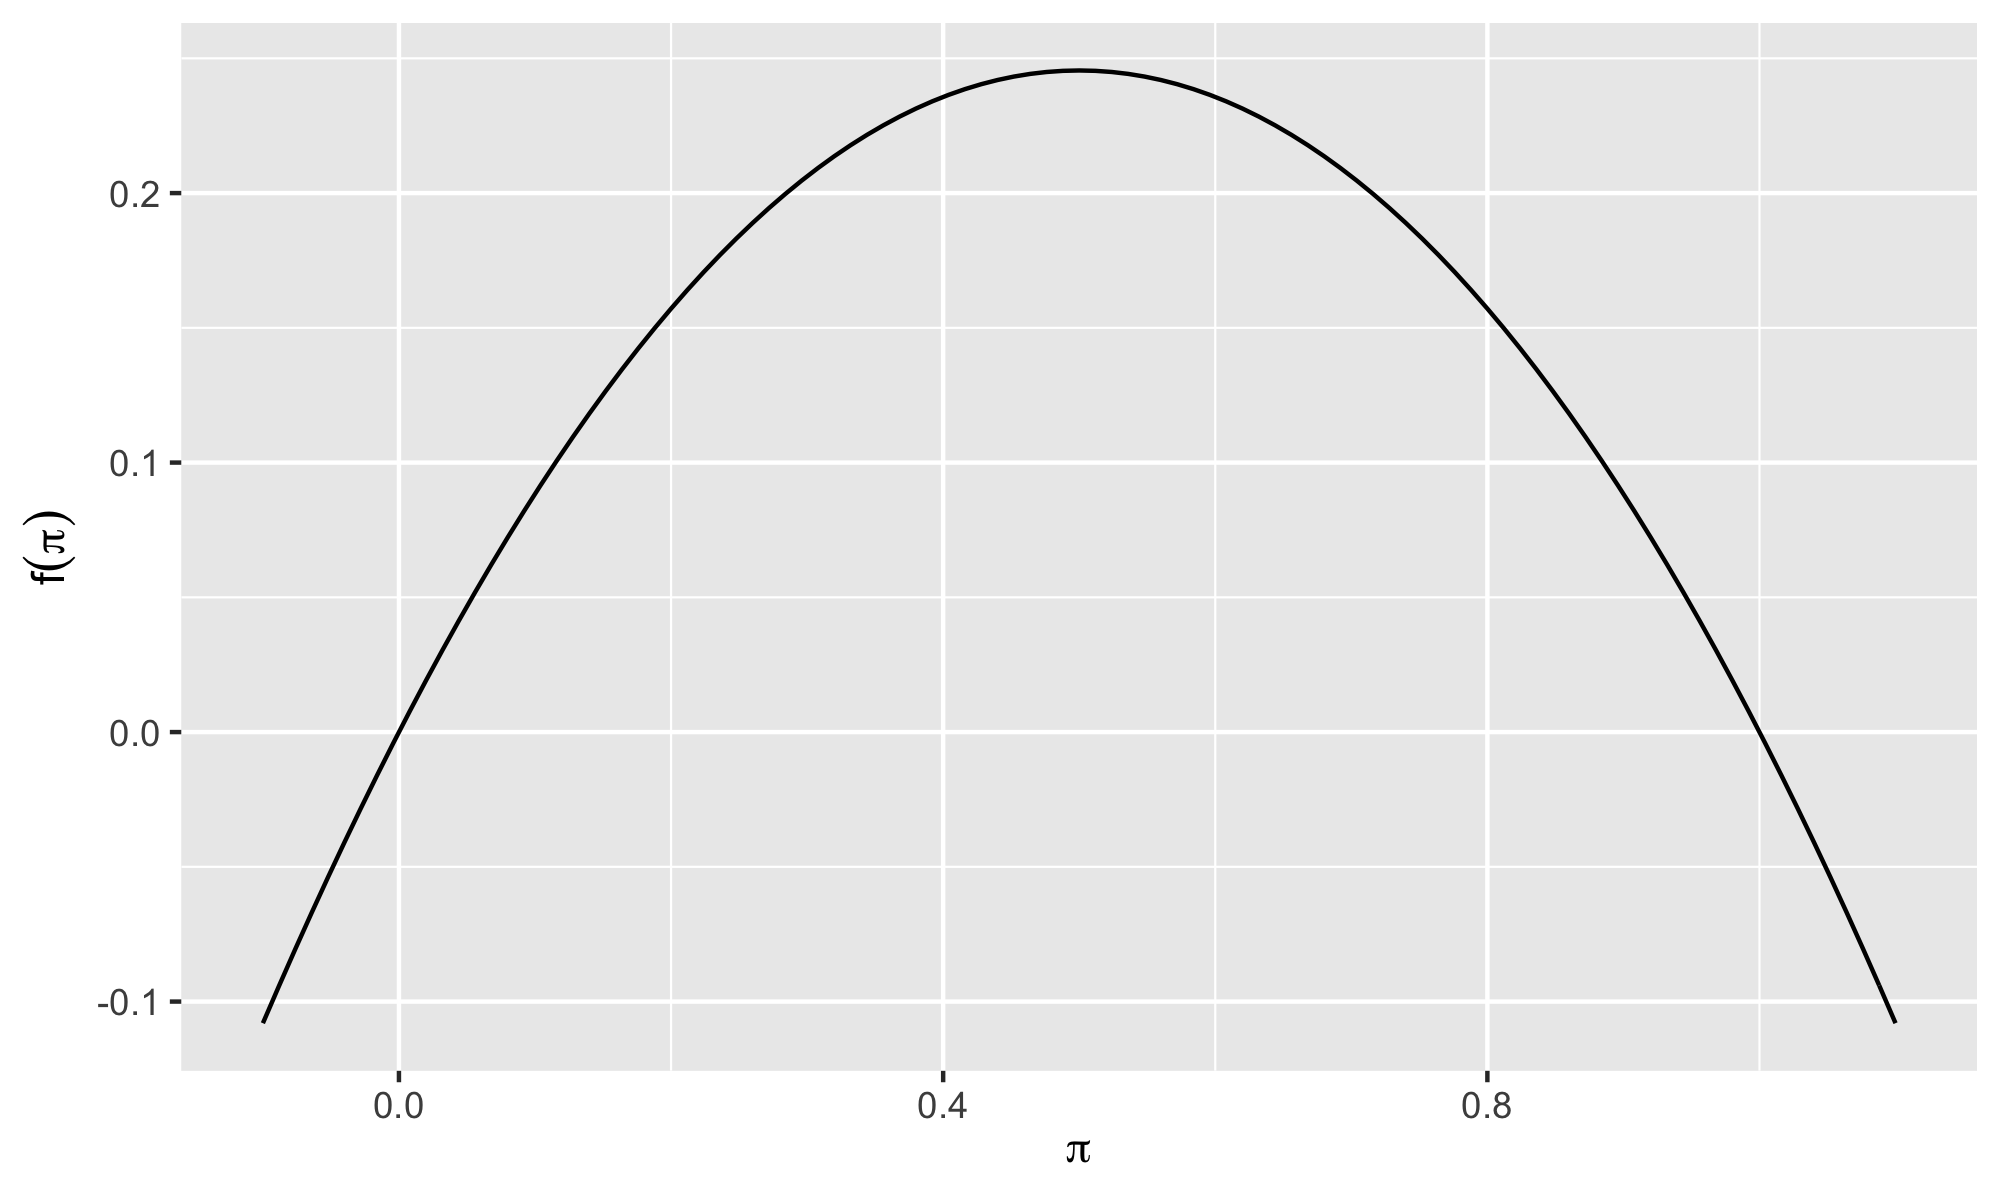
\includegraphics[width=12cm]{f-gate.png}

Similarly, \(LR(E)>1\) for any \(0< \pi <1\). Here is a plot of
\(LR(E)\) against \(\pi\):

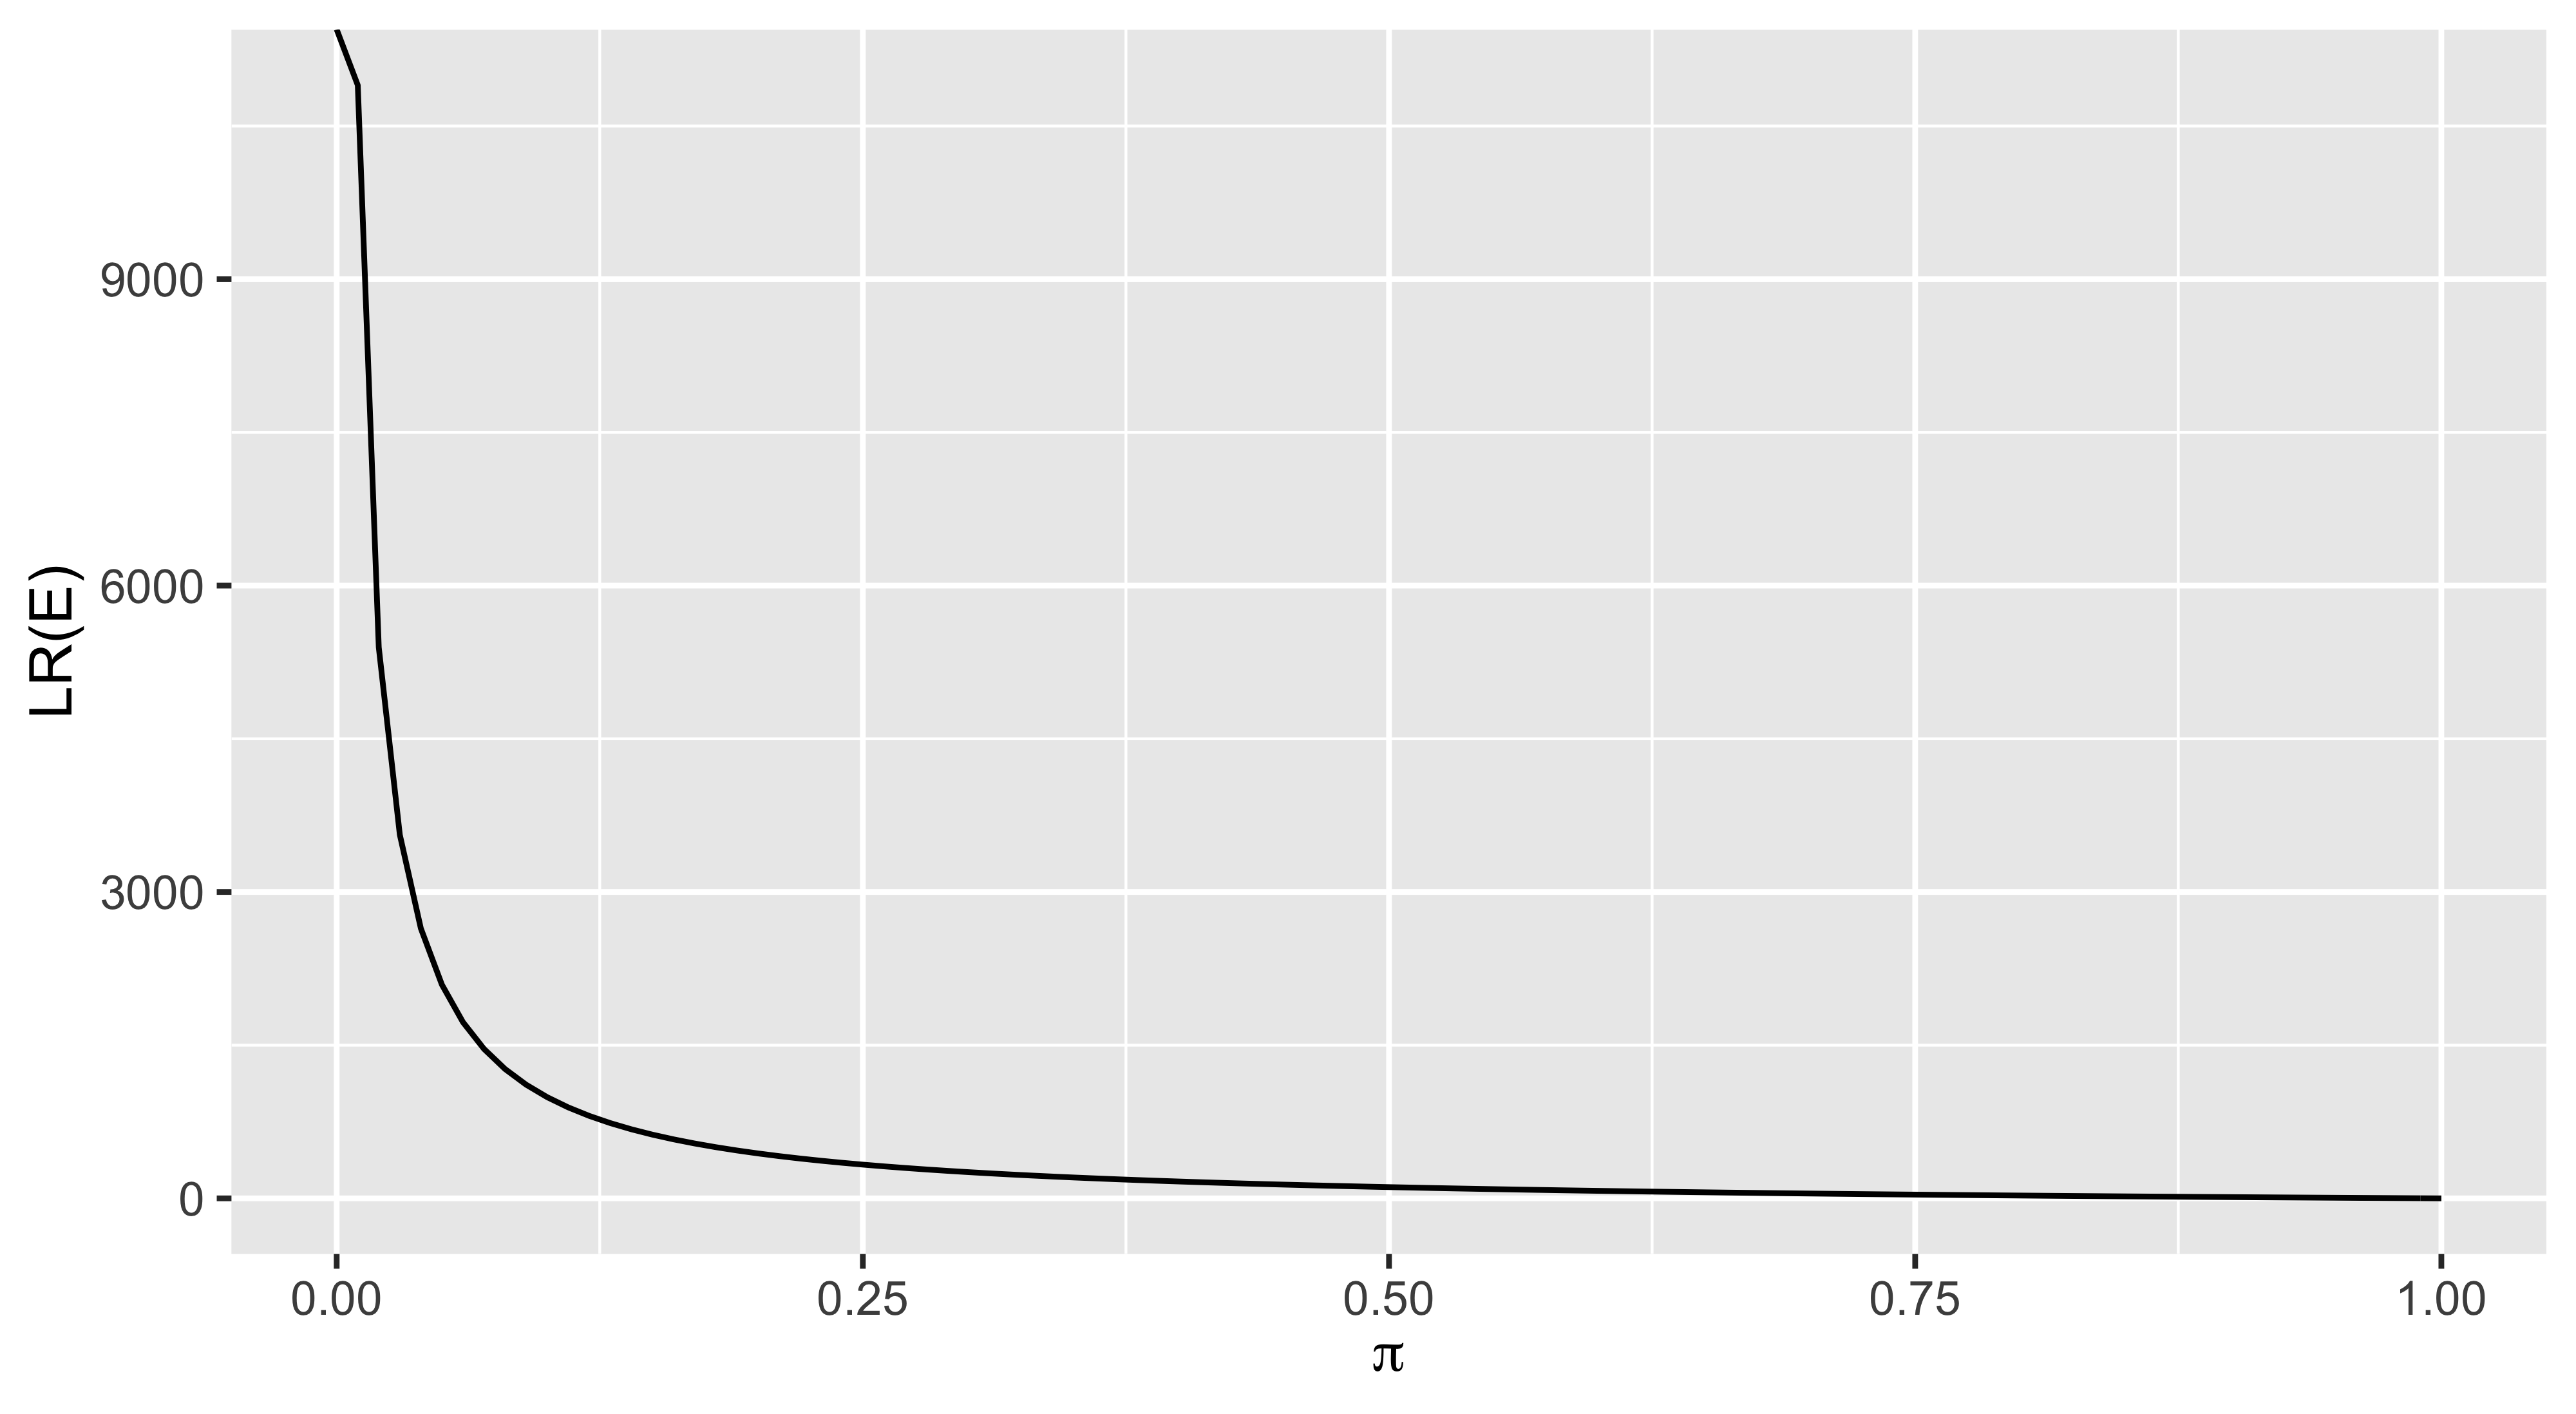
\includegraphics[width=12cm]{lre-gate.png}

\noindent Notice that \(LR(E)\) does not go below 1. This means that for
\(L=G\) in the gatecrasher scenario DTLP wold tell us to convict for any
prior probability of guilt \(\pi\neq 0,1\).

One might ask: is the conclusion very sensitive to the choice of \(L\)
and \(G\)? The answer is, not too much.

\intermezzoa

How sensitive is our analysis to the choice of \(L/G\)? Well, \(LR(E)\)
does not change at all, only the threshold moves. For instance, if
\(L/G=4\), instead of \(f\) we end up with

\begin{align*}
 f'(\pi) = - 0.955 \pi^2 + 0.955\pi &>0 
 \end{align*}

and the function still takes positive values on the interval \((0,1)\).
In fact, the decision won't change until \(L/G\) increases to
\(\approx 111\). Denote \(L/G\) as \(\rho\), and let us start with the
general decision standard, plugging in our calculations for \(LR(E)\):

\begin{align*}
LR(E) &> \frac{\pr{H_\Delta}}{\pr{H_\Pi}} \rho\\
LR(E) &> \frac{1-\pi}{\pi} \rho \\
\frac{0.991-0.991\pi}{0.009\pi} &> \frac{1-\pi}{\pi} \rho\\
\frac{0.991-0.991\pi}{0.009\pi}\frac{\pi}{1-\pi} &>  \rho\\
\frac{0.991\pi-0.991\pi^2}{0.009\pi-0.009\pi^2} &>  \rho\\
\frac{\pi(0.991-0.991\pi)}{\pi(0.009-0.009\pi)} &>  \rho\\
\frac{0.991-0.991\pi}{0.009-0.009\pi} &>  \rho\\
\frac{0.991(1-\pi)}{0.009(1-\pi)} &>  \rho\\
\frac{0.991}{0.009} &>  \rho\\
110.1111 &>  \rho\\
\end{align*}

\intermezzob

So, we conclude, in usual circumstances, DTLP does not handle the
gatecrasher paradox.

\section{Probabilistic Thresholds
Revised}\label{probabilistic-thresholds-revised}

\subsection{Likelihood ratios and naked statistical
evidence}\label{likelihood-ratios-and-naked-statistical-evidence}

\subsection{Conjcution paradox and Bayesian
networks}\label{conjcution-paradox-and-bayesian-networks}

\section{Conclusions}\label{conclusions}

Where are we, how did we get here, and where can we go from here? We
were looking for a probabilistically explicated condition \(\Psi\) such
that the trier of fact, at least ideally, should accept any relevant
claim (including \(G\)) just in case \(\Psi(A,E)\).

From the discussion that transpired it should be clear that we were
looking for a \(\Psi\) satisfying the following desiderata:

\begin{description}
\item[conjunction closure] If $\Psi(A,E)$ and $\Psi(B,E)$, then $\Psi(A\et B,E)$.
\item[naked statistics] The account should at least make it possible for convictions based on strong, but naked statistical evidence to be unjustified. 
\item[equal treatment] the condition should apply to any relevant claim whatsoever (and not just a selected claim, such as $G$).
\end{description}

Throughout the paper we focused on the first two conditions (formulated
in terms of the difficulty about conjunction (DAC), and the gatecrasher
paradox), going over various proposals of what \(\Psi\) should be like
and evaluating how they fare. The results can be summed up in the
following table:

\begin{center}
\footnotesize 
 \begin{tabular}{@{}p{3cm}p{2.5cm}p{4cm}p{3cm}@{}}
\toprule
\textbf{View} & \textbf{Convict iff} & \textbf{DAC} & \textbf{Gatecrasher} \\ \midrule
Threshold-based LP (TLP) & Probability of guilt given the evidence is above a certain threshold & fails & fails \\
Dawid's likelihood strategy & No condition given, focus on $\frac{\pr{H\vert E}}{\pr{H\vert \n E}}$ & - If evidence is fairly reliable, the posterior of $A\et B$ will be greater than the prior.

- The posterior of $A\et B$ can still be lower than the posterior of any of $A$ and $B$.

- Joint likelihood, contrary do Dawid's claim, can also be lower than any of the individual likelihoods. & fails  \\
Cheng's relative LP (RLP)
& Posterior of guilt higher than the posterior of any of the defending narrations & The solution assumes equal costs of errors and independence of $A$ and $B$ conditional on $E$. It also relies on there being multiple defending scenarios individualized in terms of  combinations of literals involving $A$ and $B$. & Assumes that the prior odds of guilt are 1, and that the statistics is not sensitive to guilt (which is dubious). If the latter fails, tells to convict as long as the prior of guilt $<0.991$. \\
Kaplow's decision-theoretic LP (DTLP) &
The likelihood of the evidence is higher than the odds of innocence multiplied by the cost of error ratio & fails & convict if cost ratio $<110.1111$
\end{tabular} 
 \end{center}

Thus, each account either simply fails to satisfy the desiderata, or
succeeds on rather unrealistic assumptions. Does this mean that a
probabilistic approach to legal evidence evaluation should be abandoned?
No. This only means that if we are to develop a general probabilistic
model of legal decision standards, we have to do better. One promising
direction is to go back to Cohen's pressure against
\textbf{Requirement 1} and push against it. A brief paper suggesting
this direction is (Di Bello, 2019), where the idea is that the
probabilistic standard (be it a threshold or a comparative wrt.
defending narrations) should be applied to the whole claim put forward
by the plaintiff, and not to its elements. In such a context, DAC does
not arise, but \textbf{equal treatment} is violated. Perhaps, there are
independent reasons to abandon it, but the issue deserves further
discussion. Another strategy might be to go in the direction of
employing probabilistic methods to explicate the narration theory of
legal decision standards (Urbaniak, 2018), but a discussion of how this
approach relates to DAC and the gatecrasher paradox lies beyond the
scope of this paper.

\section{References}\label{references}

\hypertarget{refs}{}
\hypertarget{ref-Bernoulli1713Ars-conjectandi}{}
Bernoulli, J. (1713). \emph{Ars conjectandi}.

\hypertarget{ref-buchak2014belief}{}
Buchak, L. (2014). Belief, credence, and norms. \emph{Philosophical
Studies}, \emph{169}(2), 285--311.

\hypertarget{ref-cheng2012reconceptualizing}{}
Cheng, E. (2012). Reconceptualizing the burden of proof. \emph{Yale LJ},
\emph{122}, 1254. HeinOnline.

\hypertarget{ref-Cohen1977The-probable-an}{}
Cohen, J. (1977). \emph{The probable and the provable}. Oxford
University Press.

\hypertarget{ref-cohen1988difficulty}{}
Cohen, L. J. (1988). The difficulty about conjunction in forensic proof.
\emph{The Statistician}, \emph{37}(4/5), 415. JSTOR. Retrieved from
\url{https://doi.org/10.2307/2348767}

\hypertarget{ref-dawid1987difficulty}{}
Dawid, A. P. (1987). The difficulty about conjunction. \emph{The
Statistician}, 91--97. JSTOR.

\hypertarget{ref-Dekay1996}{}
Dekay, M. L. (1996). The difference between Blackstone-like error ratios
and probabilistic standards of proof. \emph{Law and Social Inquiry},
\emph{21}, 95--132.

\hypertarget{ref-dhamiEtAl2015}{}
Dhami, M. K., Lundrigan, S., \& Mueller-Johnson, K. (2015). Instructions
on reasonable doubt: Defining the standard of proof and the jurors task.
\emph{Psychology, Public Policy, and Law, 21(2), 169178}, \emph{21}(2),
169--178.

\hypertarget{ref-DiBello2019plausibility}{}
Di Bello, M. (2019). Probability and plausibility in juridical proof.
\emph{International Journal of Evidence and Proof}.

\hypertarget{ref-diamond90}{}
Diamond, H. A. (1990). Reasonable doubt: To define, or not to define.
\emph{Columbia Law Review}, \emph{90}(6), 1716--1736.

\hypertarget{ref-finkelstein1970bayesian}{}
Finkelstein, M. O., \& Fairley, W. B. (1970). A bayesian approach to
identification evidence. \emph{Harvard Law Review}, 489--517. JSTOR.

\hypertarget{ref-Friedman2000presumption}{}
Friedman, R. D. (2000). A presumption of innocence, not of even odds.
\emph{Stanford Law Review}, \emph{52}(4), 873--887.

\hypertarget{ref-haack2011legal}{}
Haack, S. (2014). Legal probabilism: An epistemological dissent. In
\emph{Haack2014-HAAEMS} (pp. 47--77).

\hypertarget{ref-Horowitz1996}{}
Horowitz, I. A., \& Kirkpatrick, L. C. (1996). A concept in search of a
definition: The effect of reasonable doubt instrcutions on certainty of
guilt standards and jury verdicts. \emph{Law and Human Behaviour},
\emph{20}(6), 655--670.

\hypertarget{ref-Kaplan1968decision}{}
Kaplan, J. (1968). Decision theory and the fact-finding process.
\emph{Stanford Law Review}, \emph{20}(6), 1065--1092.

\hypertarget{ref-kaplow2014likelihood}{}
Kaplow, L. (2014). Likelihood ratio tests and legal decision rules.
\emph{American Law and Economics Review}, \emph{16}(1), 1--39. Oxford
University Press.

\hypertarget{ref-kaye79}{}
Kaye, D. H. (1979). The laws of probability and the law of the land.
\emph{The University of Chicago Law Review}, \emph{47}(1), 34--56.

\hypertarget{ref-kaye1986we}{}
Kaye, D. H. (1986). Do we need a calculus of weight to understand proof
beyond a reasonable doubt? \emph{Boston University Law Review},
\emph{66}(3-4).

\hypertarget{ref-Laplace1814}{}
Laplace, P. (1814). \emph{Essai philosophique sur les probabilités}.

\hypertarget{ref-laudan2006truth}{}
Laudan, L. (2006). \emph{Truth, error, and criminal law: An essay in
legal epistemology}. Cambridge University Press.

\hypertarget{ref-Nesson1979Reasonable-doub}{}
Nesson, C. R. (1979). Reasonable doubt and permissive inferences: The
value of complexity. \emph{Harvard Law Review}, \emph{92}(6),
1187--1225.

\hypertarget{ref-newman1993}{}
Newman, J. O. (1993). Beyon ``reasonable doub''. \emph{New York
University Law Review}, \emph{68}(5), 979--1002.

\hypertarget{ref-tribe71}{}
Tribe, L. H. (1971). Trial by mathematics: Precision and ritual in the
legal process. \emph{Harvard Law Review}, \emph{84}(6), 1329--1393.

\hypertarget{ref-urbaniak2018narration}{}
Urbaniak, R. (2018). Narration in judiciary fact-finding: A
probabilistic explication. \emph{Artificial Intelligence and Law},
1--32.

\hypertarget{ref-walen2015}{}
Walen, A. (2015). Proof beyond a reasonable doubt: A balanced
retributive account. \emph{Louisiana Law Review}, \emph{76}(2),
355--446.

\hypertarget{ref-wells1992naked}{}
Wells, G. (1992). Naked statistical evidence of liability: Is subjective
probability enough? \emph{Journal of Personality and Social Psychology},
\emph{62}(5), 739--752. American Psychological Association.

\end{document}
